\documentclass[12pt, a4paper]{article}\usepackage[]{graphicx}\usepackage[]{color}
%% maxwidth is the original width if it is less than linewidth
%% otherwise use linewidth (to make sure the graphics do not exceed the margin)
\makeatletter
\def\maxwidth{ %
  \ifdim\Gin@nat@width>\linewidth
    \linewidth
  \else
    \Gin@nat@width
  \fi
}
\makeatother

\definecolor{fgcolor}{rgb}{0.345, 0.345, 0.345}
\newcommand{\hlnum}[1]{\textcolor[rgb]{0.686,0.059,0.569}{#1}}%
\newcommand{\hlstr}[1]{\textcolor[rgb]{0.192,0.494,0.8}{#1}}%
\newcommand{\hlcom}[1]{\textcolor[rgb]{0.678,0.584,0.686}{\textit{#1}}}%
\newcommand{\hlopt}[1]{\textcolor[rgb]{0,0,0}{#1}}%
\newcommand{\hlstd}[1]{\textcolor[rgb]{0.345,0.345,0.345}{#1}}%
\newcommand{\hlkwa}[1]{\textcolor[rgb]{0.161,0.373,0.58}{\textbf{#1}}}%
\newcommand{\hlkwb}[1]{\textcolor[rgb]{0.69,0.353,0.396}{#1}}%
\newcommand{\hlkwc}[1]{\textcolor[rgb]{0.333,0.667,0.333}{#1}}%
\newcommand{\hlkwd}[1]{\textcolor[rgb]{0.737,0.353,0.396}{\textbf{#1}}}%
\let\hlipl\hlkwb

\usepackage{framed}
\makeatletter
\newenvironment{kframe}{%
 \def\at@end@of@kframe{}%
 \ifinner\ifhmode%
  \def\at@end@of@kframe{\end{minipage}}%
  \begin{minipage}{\columnwidth}%
 \fi\fi%
 \def\FrameCommand##1{\hskip\@totalleftmargin \hskip-\fboxsep
 \colorbox{shadecolor}{##1}\hskip-\fboxsep
     % There is no \\@totalrightmargin, so:
     \hskip-\linewidth \hskip-\@totalleftmargin \hskip\columnwidth}%
 \MakeFramed {\advance\hsize-\width
   \@totalleftmargin\z@ \linewidth\hsize
   \@setminipage}}%
 {\par\unskip\endMakeFramed%
 \at@end@of@kframe}
\makeatother

\definecolor{shadecolor}{rgb}{.97, .97, .97}
\definecolor{messagecolor}{rgb}{0, 0, 0}
\definecolor{warningcolor}{rgb}{1, 0, 1}
\definecolor{errorcolor}{rgb}{1, 0, 0}
\newenvironment{knitrout}{}{} % an empty environment to be redefined in TeX

\usepackage{alltt}
\usepackage{graphicx}
\usepackage{lipsum}
\usepackage{verbatim}
\usepackage[vmargin=3cm, hmargin=2cm]{geometry}
\usepackage{url}
\usepackage{hyperref}
\usepackage{fancyhdr}
\usepackage{color}
\usepackage{amsmath, amssymb}
\usepackage{longtable}
\usepackage{lscape}
\usepackage{natbib}
\usepackage{xspace}
\usepackage{textcomp}
\usepackage{float}
\usepackage{booktabs}
\usepackage{subcaption}
\captionsetup{font=footnotesize}
\RequirePackage{helvet}
\linespread{1.00}
\usepackage{setspace}
% =======================================
% page style
\geometry{%
  a4paper,
  top=36mm,
  left=25mm,
  right=25mm,
  bottom=24mm,
  headsep=26mm,
  footskip=15mm
}


% =======================================
% bibliography
\bibliographystyle{apalike}
\IfFileExists{upquote.sty}{\usepackage{upquote}}{}
\begin{document}

% title page
%=====================================

\thispagestyle{empty}
\renewcommand{\baselinestretch}{1.5}\normalfont
\begin{center}
\setlength{\parindent}{0cm}
\bf\Large% 
Comparison of methods for clustering of single cell RNA-sequence data \\
second line of title
\normalfont



\hrulefill

\vspace*{4cm}

\large
Master Thesis in Biostatistics (STA495)
\vspace*{12mm}

by

\vspace*{12mm}

Angelo Du\`o\\
\small 11-297-777\\
\normalfont
\vspace*{4cm}

supervised by

\vspace*{1cm}

Prof. Dr. Mark D. Robinson\\
Dr. Charlotte Soneson

\vfill

Zurich, February 2018
\end{center}
\renewcommand\familydefault{\rmdefault}%
\renewcommand{\baselinestretch}{1.0}\rm 
\setcounter{page}{0}
\cleardoublepage
%================================
\newpage\null\thispagestyle{empty}\newpage

%================================
% Abstract
\newpage
\setcounter{page}{0}

{\Large\textbf{Abstract}}\\


The aim of this thesis is to investigate the performances of clustering methods for single cell RNA sequence data. Publicly available datasets, as well as simulated datasets, are used for the comparison. The methods were tested with the gene-wise filtered and unfiltered datasets, as well as in a default run mode using default parameter settings of the methods. Several well performing methods are found, including SC3, Seurat and SIMLR. 
\newpage
%================================
% contents
\tableofcontents
\setcounter{page}{0}

%================================

\bigskip
\newpage
\setcounter{page}{1}
\section{Introduction}
Cells are one of the fundamental units of life. They show an immense complexity and diversity. Their identity and function is determined by environmental stimuli, the physical environment, the cell cycle and neighbouring cells \citep{wagner2016revealing}. Only recently has it been possible to investigate the full transcriptome of a single cell. Single-cell RNA sequencing (scRNA-seq) was first published by \citet{tang2009mrna}. This method addresses new biological issues, such as the identification of rare cell populations, and allows us to measure the frequency of cell types in tissues, characterise differences in similar cell types and investigate the heterogeneity of cell states or cell lineages \citep{andrews2017identifying}.

A typical scRNA-seq workflow consists of the isolation of single cells, the extraction of RNA, cDNA library preparation, and the amplification and sequencing of the libraries (see Figure {\ref{fig:flow}}). A wide variety of scRNA-seq protocols exists, differing in throughput, full transcript or 3' sequencing, costs and automatisation. Small-scale protocols are standard PCR plate-based methods or methods in which cell isolation and library preparation are combined into one protocol. A typical small-scale method is the PCR plate-based SMART-seq2 \citep{picelli2013smart}. Full-transcripts are sequenced using a standard Illumina approach. Typically, hundreds of cells are processed and spike-ins from the External RNA Control Consortium (ERCC) is used for normalisation. On the other side of the spectrum are droplet-based methods such as Drop-seq and 10xChromium, which allow the processing of thousands of cells.

The differences between scRNA-seq and bulk experiments are the lower sequencing depth (100,000--5 million reads per cell) compared to bulk experiments, higher variability and more outliers in the scRAnseq data. scRNA-seq data suffers from technical noise, batch effects and low capture efficiency. Confounding occurs when different biological conditions are processed in different batches, making the deconvolution of technical noise and biological effect impossible. This should be avoided by an appropriate experimental design that allows for the statistical deconvolution between unwanted and wanted variation. In scRNA-seq the single experimental unit is the cell, making it not always possible to use this approach. Different cells in an experiment may need different sample processing, or their biological differences may affect the downstream analyses.

The starting amounts of the library preparation can be as low as ten picogrammes of total RNA \citep{picelli2013smart}. Two main issues arising due to the low starting amount are  overamplification and low capture efficiency. Low and moderate expressed genes are not captured during the reverse transcription, which leads to dropouts of genes and a zero-inflated gene expression. scRNA-seq data has an excess of zero counts, which can be split into systematic, semi-systematic and stochastic zeros \citep{lun2016pooling}. Systematic zeros and semi-systematic zeros come from genes that are silent in a subpopulation or across all cells, respectively. 
Stochastic zeros are zero counts that have been obtained due to a low capture efficiency during the library preparation. They affect genes with a count distribution near zero and have to be dealt with the normalisation steps.  
 
To deal with technical noise Unique Molecular Identifiers (UMI) or spike-ins are used. UMI are short random barcodes attached to the single-stranded cDNA in the reverse transcriptase process. By counting the unique UMI reads aligned to the genome an estimated tag count is obtained. Spike-in are added before amplification. Under the assumption that the amplification of the endogenous and exogenous RNA is similar, they can be used for library size normalisation and to remove technical noise. 

In general, scRNA-seq experiments consist of high-dimensional data. High-dimensional data suffers from the curse of dimensionality \citep{wagner2016revealing}, which means the distances in high-dimensional data become unstable and subpopulations cannot be separated \citep{andrews2017identifying}. Additionally, computational requirements are high. Reduction of the dimension is made by two approaches. Using linear or non-linear projections of the data from the original high-dimensional to a lower-dimensional space, or by feature selection, in which uninformative genes are removed.

The characterizing of of the composition in a sample is one of the most common aims for scRNA-seq data. Lately, a broad spectrum of clustering methods have been specifically developed for the clustering of single cells. The aim of this study is to evaluate clustering methods for scRNA-seq data.

\paragraph{Aims of the study}

Several methods for clustering exists, but up to now no comparison study testing the methods independently is known.
The aim of the study is the comparison of clustering methods for scRNA-seq data. For the evaluation, publicly available datasets are used, providing a range of the sequencing depth, dropout fractions, type of expression values, number of subpopulations and difficulty of the dataset. Whereas these datasets provide the means to test the clustering methods on realistic data it has the disadvantage of unknown ground truth. To circumvent this, simulated datasets will be considered, enabling the evaluation of the clustering results on a secured ground truth of the clusters labels.  Due to the high-dimensionality and large technical variation of scRNA-seq data, filtering and normalisation are crucial steps in the clustering workflow. Here we want to investigate the effect of clustering using genewise filtered and unfiltered datasets. Another aim is to test the methods in the default mode by using the default settings of the methods with a minimum required user effort. This is considered as important as many users will use the methods without any finetuning of the methods.
Finally, also the runtime and the stability of the methods is investigated.

\begin{figure}[!h]
\begin{center}
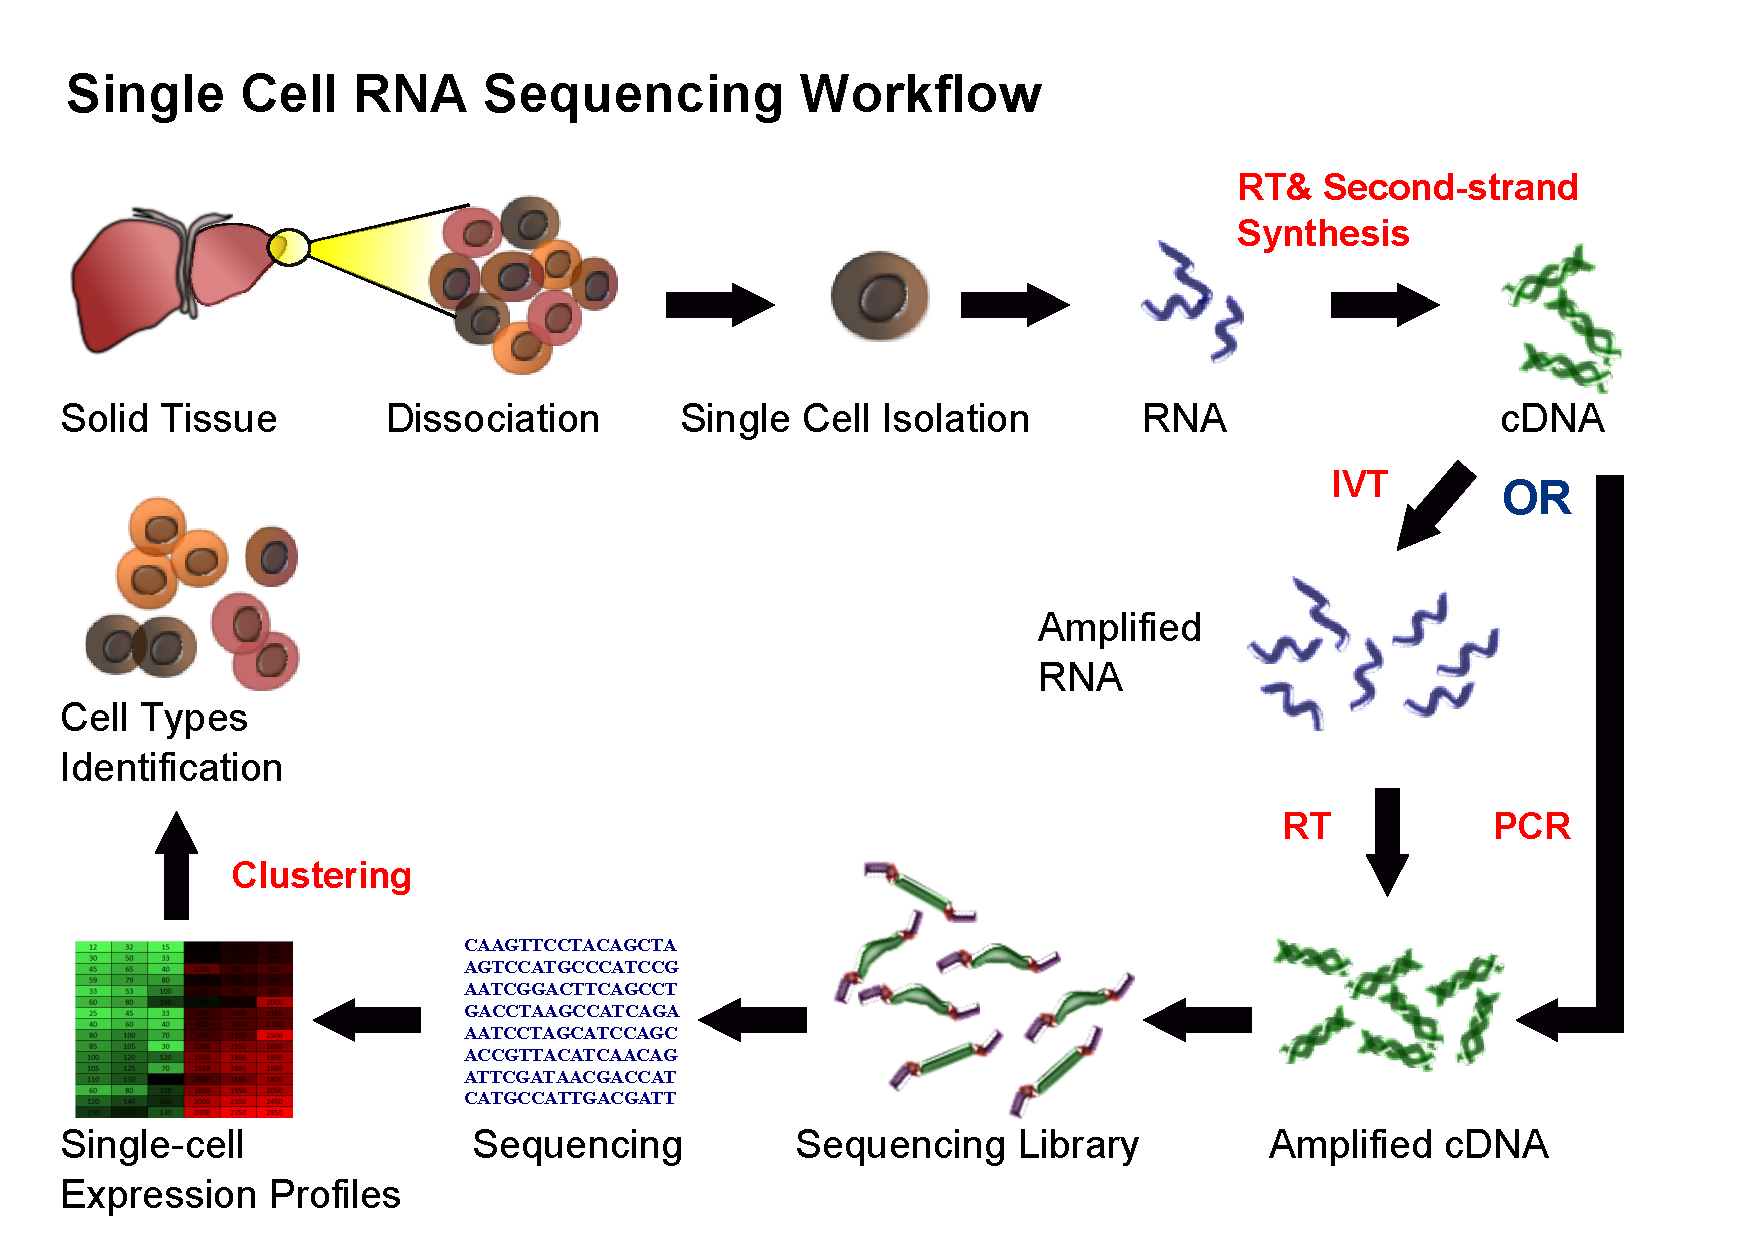
\includegraphics[width=5 in]{/Users/angeloduo/Desktop/masterarbeit/scRNAseq_clustering_comparison/report/figures/RNA-Seq_workflow.pdf}
\caption{Single-cell RNA sequencing workflow. The workflow consists of the following steps: the isolation of the single cells and RNA, reverse transcription of the RNA to cDNA and the subsequent amplification, library preparation and sequencing. Taken from Wikipedia. }

\label{fig:flow}
\end{center}
\end{figure}

\clearpage

\newpage

\section{Methods}

\subsection{Dimension reduction}

All methods require a dimension reduction step before clustering. Commonly used methods are either Principal Component Analysis (PCA) \citep{hotelling1933analysis} or t-distributed Stochastic Neighbour Embedding (tSNE). Given a data matrix $X (nxp)$ with $n$ measurements and $p$ random variables, and we want to reduce the dimension from $p$ to $q$ random variables. Then, PCA finds the linear combinations $a_{1}x^T, a_{2}x^T,\ldots, a_{q}x^T$ which have the succesive maximum variance, subject to the constraint that its sample correlations with previous $a_{k}x^T$ equals zero.
Or in other words, PCA finds a orthogonal rotation of the original data in which the newly obtained first coordinates have the highest possible variance, the second coordinates the second-greatest variance etc. The linear combinatios are the so called principal components.
Practically, PCA is computed by spectral decomposition of the correlation $R$ or covariance matrix $S$. The vectors $a_{1}, a_{2},\ldots, a_{q}$ are the eigenvectors of $S$ corresponding to the $q$ largest eigenvalues \citep{jolliffe1986principal}.  Dimension reduction is achieved either by selecting only the first few PCs whose eigenvalues are above the average, or by determining the number graphically by plotting the eigenvalues (scree plot). PCA is deterministic and relatively fast but restricted to linear spaces.

In contrast,  tSNE is a non-linear mapping \citep{van2013barnes}. Stochastic neighbour embedding (SNE) transforms Euclidean distances to conditional probabilities $p_{j|i}$. That is the probability that \(x_j\) is the nearest neighbour of $x_i$ under a Gaussian centred at $x_i$. The low-dimensional counterpart $q_{i|j}$ is similar with a Gaussian centered at $y_i$ and variance of $1/\sqrt(2)$. SNE minimises the divergence between $p_{j|i}$ and $q_{j|i}$ using the Kullback-Leibler divergence. tSNE implements a Student's t-distribution for the low dimensional space and a symmetric version of the cost function to simplify optimisation and to overcome the crowding problem. In tSNE, the cost function uses the joint probabilities $p_{ij}$ and $q_{ij}$ instead of conditional probabilities. To deal with large datasets, the Barnes-Hut implementation uses random walks on the nearest neighbour network with a PCA step to reduce the dimensionality of the high-dimensional data. tSNE is stochastic, depends on a perplexity parameter and distances between clusters are not preserved. 
\subsection{Clustering methods}
Identifying unknown cell populations is one of the main uses of scRNA-seq data \citep{andrews2017identifying}. Eleven clustering methods have been evaluated for this study. These methods and algorithms can be roughly classified into three groups: K-means, graph-clustering and hierarchical-based clustering. 
SC3, SIMLR, Linnorm and RaceID use k-means in different fashions, while pcaReduce and CIDR are based on hierarchical clustering. The graph-based methods are SNN-Cliq and Seurat. An overview of the methods is given in Table \dots


% Table generated by Excel2LaTeX from sheet 'Blatt1'
\begin{table}[htbp]
  \centering
  \caption{Add caption}
   \resizebox{\textwidth}{!}{%
    \begin{tabular}{p{6.915em}p{14.915em}p{5.085em}p{10.25em}p{2.665em}p{4.165em}p{4.415em}}
    \toprule
    \multicolumn{1}{l}{\textbf{Method}} & \multicolumn{1}{l}{\textbf{Description}} & \textbf{dimension reduction} & \multicolumn{1}{l}{\textbf{clustering}} & \multicolumn{1}{l}{\textbf{dropout}} & \multicolumn{1}{l}{\textbf{normalization}} & \multicolumn{1}{l}{\textbf{unsupervised}} \\
    \midrule
    \textbf{tSNEkmeans} & tSNE dimension reduction and kmeans clustering & tSNE  & k-means & no    & no    & no \\
    \midrule
    \textbf{pcaReduce} & PCA dimension reduction and k-means clustering through an iterative process. Step wise merging  of  cluster by joint probabilities and reducing the  number cof dimension by PC with lowest variance. & PCA   & k-means, hierarchical clustering & no    & no    & yes \\
    \midrule
    \textbf{SC3} & PCA   dimension   reduction   or Laplacian    graph. k-means clustering on different dimensions.  Hierarchical clustering on consensus matrix   obtained by k-means & PCA   & repeated k-means, hierarchical clustering on similarity matrix of k-means & no    & no    & yes \\
    \midrule
    \textbf{SNNCliq} & Shared  nearest  neighbor  graph based on similarities. Clustering through forming of cliques  and subsequent merging. & graph based & merging of cliques & no    & no    & no \\
    \midrule
    \textbf{SIMLR} & Learning of a distance metric via multiple kernel learning & tSNE  & k-means & yes   & no    & yes \\
    \midrule
    \textbf{CIDR} & PCA dimension reduction based on zero imputed similarities.  Hierarchical clustering on a number of PC determined by variation of scree method. & PCA   & hierarchical clustering & yes   & no    & yes \\
    \midrule
    \textbf{Seurat} & Nearest neighbor graph based on PCA latent space & HVG and PCA & graph based & no    & yes   & yes \\
    \midrule
    \textbf{TSCAN} & Ordering of cells by the use of a TSP algorithm. & PCA   & graph based & no    & yes   & no \\
    \midrule
    \textbf{Linnorm} & Normalisation using a subset of genes and clustering through tSNE/PCA and k-means & tSNE and k-means & k-means & yes   & yes   & yes \\
    \midrule
    \textbf{RaceID} & Filtering and normalisation of cells and clustering with k-means. & -     & k-means & no    & yes   & yes \\
    \bottomrule
    \end{tabular}}%
  \label{tab:addlabel}%
\end{table}%


\paragraph{K-means}
K-means clustering finds a predefined number of centres $k$ and cell assignments, such that their within-group sum of squares is minimised \citep{hartigan1979algorithm}. $k$ cluster centres are randomly assigned.
Each data point is then assigned to the nearest centre using Euclidean distances. The centres are then recomputed using the average of the data points that are assigned to each of the $k$ centres. This procedure is iterated until the algorithm converges. The assigning of the centres is random. Also, it's not guaranteed to find the global minimum.  The drawbacks of the method are that it assumes spherical clusters and this is sensitive to scaling. 
\paragraph{pcaReduce}
pcaReduce uses k-means clustering to find the number of clusters in the reduced dimension given by PCA \citep{yau2016pcareduce}. The main assumption is that large classes of cells are contained in low-dimension PC representation and more refined subsets of these cells types are contained in higher-dimensional PC representations. Given a gene expression matrix, the clustering algorithm starts with a k-means clustering on the PCA projections $Y_{n\times q}$ with $q+1$ clusters, where $n$ is the number of cells and $q$ are the number of PCs. The number of initial clusters $k$ is typically around 30,  guaranteeing that most cell types are captured. For all pairs of clusters, the joint probabilities are computed. Two clusters are merged by selecting the pair with the highest joint probability or by sampling proportionally by the joint probabilities. The number of clusters is now decreased to $k-1$. Next, the PC with the lowest variance is deleted and a k-means clustering with $k-2$ centers is performed. This process is repeated until only one single cluster remains. When using pcaReduce $q$ cluster partitions with $k-1$ clusters are obtained. The user can than choose the clustering with the desired number of clusters.
\paragraph{SC3}
Implemented in the SC3 method is gene- and cell-filtering, as well as a log transformation step of the expression matrix \citep{kiselev2017sc3}. The filtered expression matrix is then used to compute  Euclidean, Pearson and  Spearman dissimilarity measures. By PCA or Laplacian graphs a lower-dimensional representation of the data is obtained.  K-means clustering is then performed on the different dimensions. Next, a consensus matrix of the different clustering results is computed. The consensus matrix is a binary similarity matrix with entry one if two cells belong to the same cluster and zero otherwise. The consensus matrix is obtained by averaging the individual clustering. The last step is a hierarchical clustering step with complete linkage. The cluster is inferred by the $k$ level of hierarchy, where $k$ can be supplied by the user. The method allows for the estimation of $k$. (Using the covariance matrix of the expression matrix the function finds the eigenvalues. The Tracy-Widom test is used for estimating the number of significant eigenvalues, which represent the number of estimated $k$. )
To reduce runtime, SC3 changes the clustering method when supplied with more than 5'000 cells. Randomly selected cells are then used for the clustering approach described above. These subpopulations are then used to train a support vector machine to infer the cluster labels of the remaining cells.
\paragraph{SNNcliq}
SNNcliq computes a shared nearest-neighbour-graph based on the high-dimensional data \citep{xu2015identification}. The nodes are the data points and the weighted edges are the similarities between the data points. Cells are defined as a cluster if they have a defined number of edges between them, forming a "clique". 

A similarity matrix using Euclidean or other similarity measures is then computed. Using this similarity matrix, the k-nearest-neighbours (KNN) for each data point are listed. The number of nearest neighbours has to be supplied by the user. Edges between data points are assigned if they share at least one KNN. The weights of the edges are defined by a function of the number of nearest neighbours and their respective ranks. 
Identification of clusters is made by finding quasi-cliques associated with each node and merging them to unique clusters by the use of a greedy algorithm. A node induces a subgraph, which consists of all neighbour nodes and edges. For each node, a local degree is computed and a node is removed from the subgraph if its degree is lower than a given threshold which is proportional to the size of the clique. The threshold is supplied by the user and is typically set to 0.7. Next, the degrees between the nodes are recomputed and the process is repeated until no more nodes can be removed. A subgraph is assigned to a quasi-clique if it contains more than three nodes. To reduce redundancy, quasi-cliques that are completely included in other cliques are removed as well.
Clusters are then identified by merging the quasi-cliques. For each pair, an overlapping rate is computed. If it exceeds a predefined threshold $m$ the subgraphs are merged. Merging in different orders leads to different results, so pairs with larger sizes are prioritized.
\paragraph{SIMLR}
Most clustering methods rely on standard similarity metrics like Euclidean distances \citep{wang2017visualization}. SIMLR uses a weighted function of multiple kernels to compute a distance matrix. The assumptions is that the matrix has a block-diagonal structure, where the blocks represent the clusters $c$. The kernels are Gaussian kernels with a range of hyperparameters defining the variance of each kernel. The similarities are then used for data visualisation with tSNE or clustering using k-means on the latent space representations of the similarities.

\paragraph{CIDR}
Clustering through Imputation and Dimensionality Reduction (CIDR) takes the high dropout rate in scRNA-seq data into account \citep{lin2017cidr}. The method splits the squared Euclidean distance into three terms. These consist of one term in which both genes $k$ for the cell pairs $i$ an $j$ are non-zero, a second term in which one gene is zero and a third where both are zero. The authors state that only the cases where one gene is zero have a strong influence on the distances and the subsequent dimension reduction and clustering. To reduce the dropout-induced zero inflation, the method imputes the third term by its expected value given the distribution of the dropouts. 
The algorithm works basically in five steps: (i) Find features that are dropout candidates. That is genes that show an expression level below a threshold $T$. (ii) Find the empirical dropout probability $\hat P(u)$ using the whole data set. (iii) Calculate the dissimilarity using Euclidean distances together with a pairwise imputation process. Features that fall below the threshold $T$ are imputed using a weighting function. The weighting is based on the probability of being a dropout. (iv) Perform dimension reduction using PCA on the imputed distance matrix. (v) Perform hierarchical clustering using the first few PCs. The number of PCs can be determined by several methods. Here, we use an implemented variation of the scree method. 
\paragraph{Linnorm }
Linnorm is a normalisation and transformation method for count data \citep{yip2017linnorm}. The main assumption is that a homogeneously expressed gene-set exists. Using this gene subset, and by ignoring zero counts, the normalisation and transformation parameters are calculated. After normalisation, the expression values should show both homoscedasticity and normality. Linnorm includes functions for subpopulation analysis by t-SNE or PCA dimension reduction and subsequent k-means or hierarchical clustering. 

First, the values are scaled according to library size. Low count genes and genes that show high technical noise are filtered out. By default, genes showing a non-zero expression in at least 75 \% of the cells are retained. Note that this threshold is set to maintain at least three non-zero cells per gene, in order to calculate the skewness of the gene distributions. By gradually increasing this threshold only genes that show a negative correlation between the mean and the standard deviation (SD) is assured. 
A locally weighted scatterplot smoothing (LOWESS) curve is fitted on the mean versus SD relationship. The SD is scaled and outliers based on the SD are removed. Next, genes that show a high skewness are filtered out. The data is then transformed using a modified log transformation.
The dimensions are reduced by PCA or tSNE and clustering using the k-means algorithm. The R packages fpc, vegan, mclust and apcluster are used to determine the number of clusters.

\paragraph{TSCAN}
TSCAN uses a pseudo-time algorithm for cell ordering \citep{ji2015tscan}. PCA dimension reduction on the preprocessed gene expression data is performed. Preprocessing is done by log transformation and by adding a pseudo-count. Low expressed genes are filtered out based on the zero-proportion and their covariance. Clustering is done by model-based clustering. 
The travelling salesman problem (TSP) is then solved by a minimum spanning tree. The user can then define the start/end point through the available biological information and compute a pseudo-time ordering score. 
\paragraph{RaceID}
Rare Cell Type IDentification (RaceID) is a method developped for the data preprocessing, detection of outlier cells, k-means clustering and the inference of rare subpopulations. Cells are filtered based on a minimum number of transcripts. The expression matrix is normalised by scaling by the library size. To ensure non-zero values a pseudocount of 0.1 is added to the expression data.
Using genefilter genes with a high zero-proportion are filterd out as well.
The implented clustering function uses k--means and the clusterboot function from the R package fpc for clustering. In contrast to the originial k-means clustering in clusterboot, the newly developped function can use not only euclidean distances. 
The number of clusters is determined by the use of the gap statistic implemented in the clusterboot function.

The authors state that the algorithm is based on absolute transcript counts and is not tested for datasets containing other expression values than counts. With respect datasets other than the Zheng data the results should be interpreted carefully.

\paragraph{Seurat}
Seurat uses raw counts, where filtering is both done gene- and cell-wise. A user-specified threshold for the minimum number of expressed features per cell and the minimum number of the gene-wise expression per cell has to be defined. The counts from each cell are normalised by their total counts, scaled by a factor of 10000 and log-transformed. A set of high-variable genes (HVG) is found by calculationg the average expression and dispersion for each gene. Based on the average expression the genes are divided into bins. Within each bin z-scores for the dispersion is calculated. The HVG are then selected by their standart deviation.
Dimension reduction is done by PCA. The number of PCs is deterimed by a permutation test or graphically by plotting the eigenvalues of the PCs. Clustering is graph-based using a KNN-graph of the euclidean distances in the PCA space. Clustering of cells is done by the Louvain algorithm \citep{butler2017integrated}.
\paragraph{ZINBWaVE}
Zero-inflated Negative Binomial-based Wanted Variation Extraction (ZINB-WaVE) uses zero-inflated negative binomial model to model the count data\citep{risso2017zinb}. By using the a zero-inflated negative binomial model the dropouts and over-dispersion is taken into account. It allows for the inclusion of cell-level and gene-level covariates, such as batch effects or quality control measures. Included are also unobserved sample-level covariates, these are inferred from the data and can represent the unwanted variation or the biological effects of interest. The parameter estimation is done throug a penalized likelihood approach. ZINB-WaVE can be used for a low-dimensional representation of the data and clustering is done by the use of kmeans.

\newpage
\subsection{Datasets}
The datasets Kumar, Trapnell and Koh were downloaded from the \textit{conquer} repository \url{http://imlspenticton.uzh.ch:3838/conquer}. 
The Zheng data was downloaded from the 10xChromium repository: \url{https://support.10xgenomics.com/single-cell-gene-expression/datasets}. For the Kumar, Trapnell and Koh data count-scale Transcripts Per kilobase Million (TPM) are used.  These are on a count-scale and are independent from the average length of the transcript \citep{soneson2015differential}. The Zheng data consists of UMI counts. Figure \ref(fig:datatsne) shows the datasets in the tSNE space. Table \ref{tab:data} shows several summary statitistic of the datasets. To have a measure of the compactness and difficulty of the datasets the silhouette width were computed. Reported are the average silhouette widths for each dataset.

\paragraph{\citet{kumar2014deconstructing}}
The Kumar dataset consists of $Dgcr8$-knockout and V6.5 variotypes from mouse embryonic stem cells (mESCs). Cells were cultured on a serum with a Leukaemia Inhibitory Factor (LIF) or under Erk and GSK3 signalling inhibition (2Li). The authors investigated the expression of pluripotency factors and their involvement in the heterogeneity of pluripotent stem cells. Sample preparation and whole transcriptome amplification was done using a Fluidigm C1 system and following a SMARTer protocol. Sequencing was done using the Illumina system with paired-end reads. Sequencing depth was 1 million reads per cell.
\paragraph{\citet{trapnell2014dynamics}} 
\citet{trapnell2014dynamics} used human skeletal muscle myoblast cells to investigate temporal differentiation. Cells were expanded under high--mitogen conditions. Differentiation was induced by switching to low-serum medium. Cells were captured before switching to low-serum medium (T0), after 24 h (T24) and 48h (T48). Between 49 and 77 cells were isolated at each time point and used for single mRNA-Seq library preparation by the use of a Fluidigm C1 system and following a SMARTer protocol. Libraries were sequenced with paired-end sequencing on a HiSeq 2500 (Illumina) platform. Sequencing depth was ˜4 million reads per library. The authors excluded libraries that contained fewer than 1 million reads. 
\paragraph{\citet{koh2016atlas} }
H7 human embryonic stem cells (hESCs) were used to study human mesoderm development. Starting from undifferentiated stem cells, several differentiation stages, sorted by time point and further refined by fluorescence-activated cell sorting (FACS) were isolated. Finally, nine different cell lines were obtained:  undifferentiated H7 hESCs (H7hESC), anterior primitive streak populations (APS), mid primitive streak populations (MPS), lateral mesoderm (D2LtM), FACS-purified DLL1+ paraxial mesoderm populations (DLL1pPXM), early somite progenitor populations (ESMT), PDGFRα+ sclerotome populations (Sclrtm) and two different dermomyotome populations (D5CntrlDRmmtm).
In total, ten different cell types were then sequenced on a Fluidigm C1 system and following a SMARTer protocol. Libraries were sequenced through paired-end sequencing on a HiSeq 2500 (Illumina) platform. Sequencing depth was 1 -- 2 million reads per cell. 
\paragraph{ \citet{zheng2017massively}}
FACS-purified fresh peripheral blood mononuclear cells (PBMCs) were used to assess the performance of the 10xChromium system. Sample preparation and library construction were done with a 10xChromium system. The libraries were sequenced using an Illumina system. For this study, the datasets for CD19+B, CD8+CD45RA+ naive cytotoxic, CD14+ monocytes and CD4+/CD25+ regulatory T cells were used to construct an artificial population. From each library, 200 cells were sampled before being merged to obtain a single expression matrix.
\paragraph{Simulated datasets }
Using the Splatter package, expression data were simulated \citep{oshlack2017splatter}. Parameters for the simulation were estimated from a subpopulation of the Kumar dataset.  Embryonic stem cell variotypes V6.5 with signalling inhibition and LIF were used for the estimation. SimDataKumar consists of 500 cells with four subpopulations. The fractions per subpopulations were 0.1, 0.15, 0.5 and 0.25 of the total cell population. The probability that a gene is differentially expressed is 0.05, 0.1, 0.2 and 0.4 in the four different groups. Similarly, SimDataKumar2 consists of four subgroups with fractions of 0.2, 0.15, 0.4 and 0.25 of a total of 500 cells. The fractions of differentially-expressed genes were lower, with a probability of 0.01, 0.05, 0.05 and 0.08. The spike-in RNA is excluded before the parameter estimation.
\begin{figure}[!h]
\begin{center}
\includegraphics[width= 7 in]{/Users/angeloduo/Desktop/masterarbeit/scRNAseq_clustering_comparison/results/QC_data/plot_data_tsne.pdf}
\caption{tSNE representation of the datasets (a) Kumar , (b) Trapnell, (c) Zheng, (d) Koh, (e) simDataKumar and (f) simDataKumar2 . The subpopulations in the datasets are color coded.  }
\label{fig:datatsne}
\end{center}
\end{figure}


% Table generated by Excel2LaTeX from sheet 'Blatt1'
\begin{table}[htbp]
  \centering
  \caption{Summary statistics of the datasets. Shown are the number of cells, the number of subpopulations, the median library size, the median total read counts and the average silhouette widths.}
   \resizebox{\textwidth}{!}{%
    \begin{tabular}{llcccccl}
    \toprule
    \multicolumn{1}{p{6.915em}}{\textbf{Dataset}} & \multicolumn{1}{p{6.665em}}{\textbf{Sequencing Method}} & \multicolumn{1}{p{4em}}{\textbf{No of cells}} & \multicolumn{1}{p{6.665em}}{\textbf{Median library size }} & \multicolumn{1}{p{7.585em}}{\textbf{Median total counts (mio)}} & \multicolumn{1}{p{6.25em}}{\textbf{Avg. silhouette}} & \multicolumn{1}{p{6.25em}}{\textbf{No of subpopulations}} & \multicolumn{1}{p{8.585em}}{\textbf{Ref.}} \\
    \midrule
    \textbf{Kumar} & SMARTer & 268   & 25,894 & 1.67  & 0.53  & 3     & \textit{Kumar et. al (2014)} \\
    \textbf{Trapnell} & SMARTer & 288   & 13,616 & 1.86  & 0.04  & 3     & \textit{Trapnell et. al (2014)} \\
    \textbf{Zheng} & 10xChromium & 2000  & 489   & $<$ 0.01 & 0.1   & 4     & \textit{Zheng et al. (2017)} \\
    \textbf{Koh} & SMARTer & 651   & 13,765 & 1.3   & -0.04 & 10    & \textit{Koh et al. (2016)} \\
    \textbf{simDataKumar} & -     & 500   & 29,861 & 1.78  & 0.15  & 4     & - \\
    \textbf{simDataKumar 2} & -     & 500   & 29,974 & 1.78  & 0.03  & 4     & - \\
    \bottomrule
    \end{tabular}}%
  \label{tbl:data}%
\end{table}%



\begin{figure}
\centering
\begin{subfigure}{.5\textwidth}
  \centering
  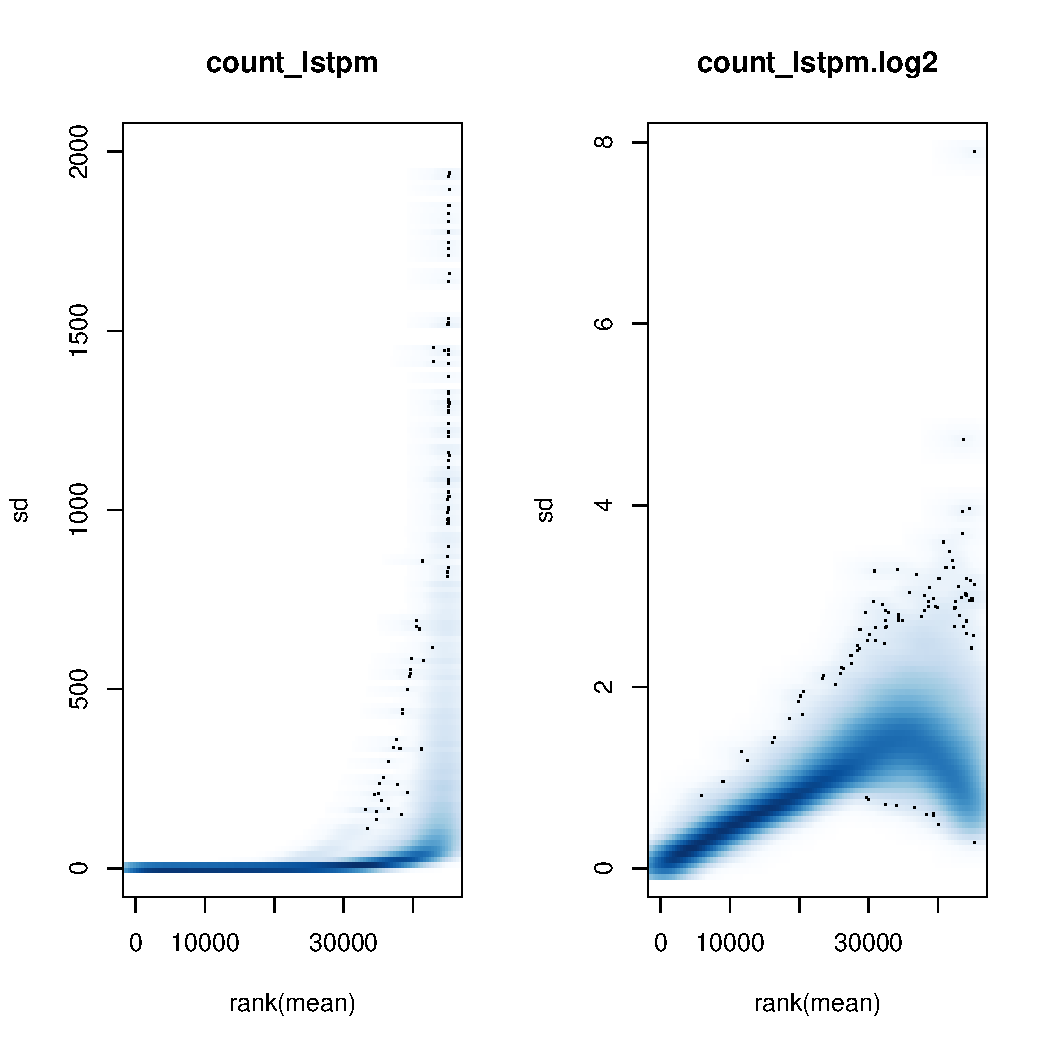
\includegraphics[width=1\linewidth]{/Users/angeloduo/Desktop/masterarbeit/scRNAseq_clustering_comparison/results/QC_data/meanvarplots_kumar2015.pdf}
  \caption{Kumar dataset}
  \label{fig:transsim}
\end{subfigure}%
\begin{subfigure}{.5\textwidth}
  \centering
  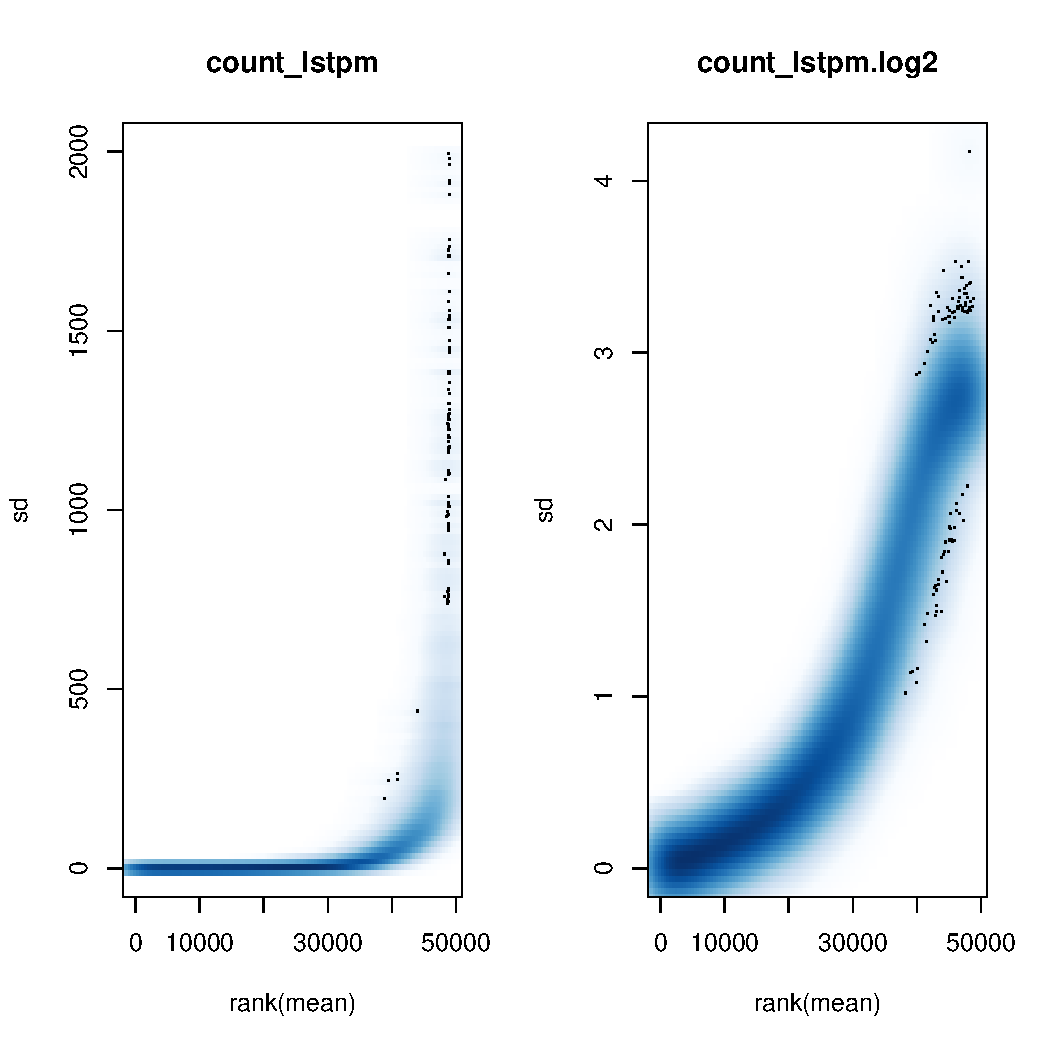
\includegraphics[width=1\linewidth]{/Users/angeloduo/Desktop/masterarbeit/scRNAseq_clustering_comparison/results/QC_data/meanvarplots_koh2016.pdf}
  \caption{Koh dataset}
  \label{fig:transkoh}
\end{subfigure}
\begin{subfigure}{.5\textwidth}
  \centering
  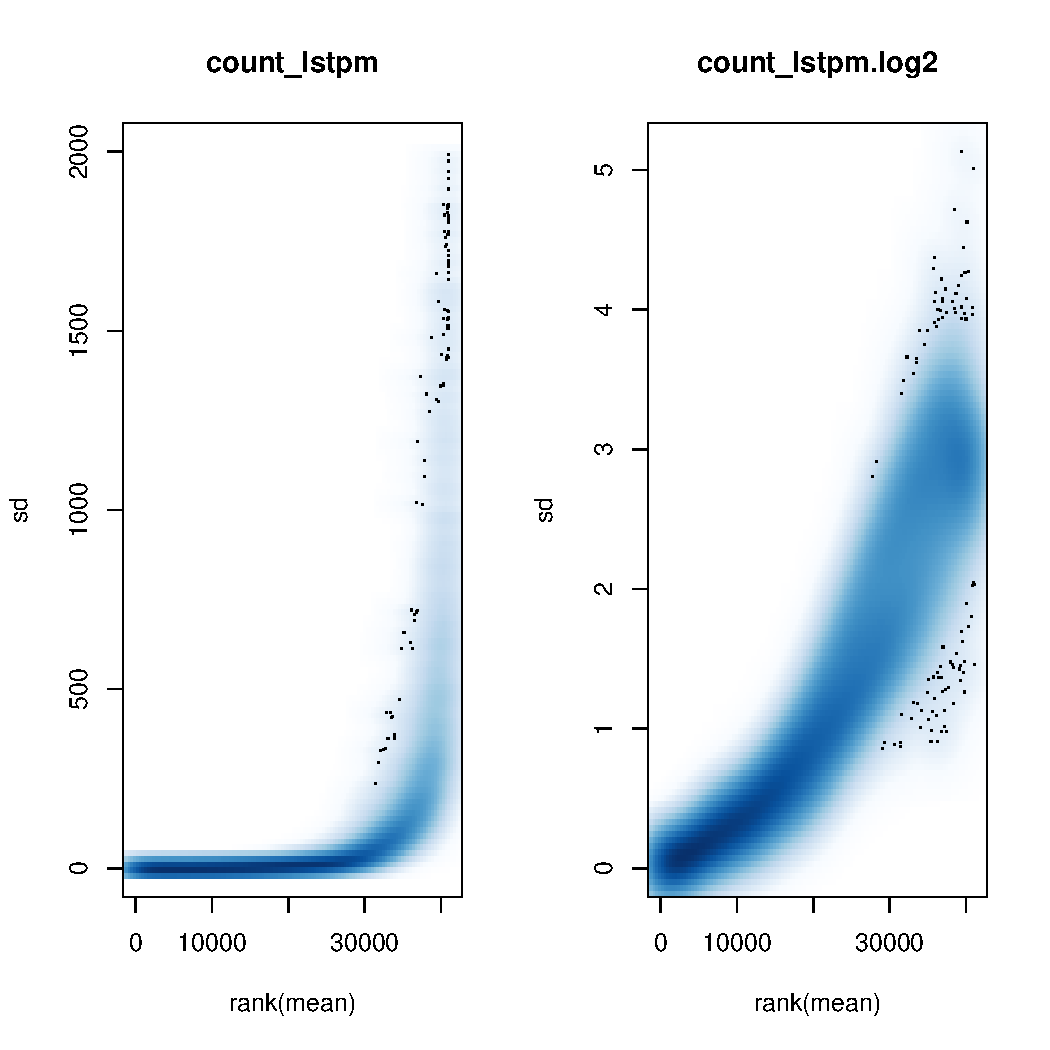
\includegraphics[width=1\linewidth]{/Users/angeloduo/Desktop/masterarbeit/scRNAseq_clustering_comparison/results/QC_data/meanvarplots_trapnell2014.pdf}
  \caption{Trapnell dataset}
  \label{fig:transtrapnell}
\end{subfigure}%
\begin{subfigure}{.5\textwidth}
  \centering
  \includegraphics[width=1\linewidth]{/Users/angeloduo/Desktop/masterarbeit/scRNAseq_clustering_comparison/results/QC_data/meanvarplots_zhengmix2016.pdf}
  \caption{Zheng dataset}
  \label{fig:transzheng}
\end{subfigure}
\caption{Shown is the genewise standart deviation versus the mean for the datasets Kumar (a), Koh (b), Trapnell (c) and Zheng (d). Different transformations were considered; log, arcus sin and VST transformations. }
\label{fig:trans}
\end{figure}

\newpage
\subsection{Data transformation and normalisation}\label{ssec:norm}
\paragraph{Data transformation}
RNA-seq data may suffer from heteroscedasticity and skewness \citep{zwiener2014transforming}. Genes with higher mean have on average a higher variance across cells leading to unequal variances between different genes. 
To handle this property different transformation were considered. Namely, a binary logarithmic transformation with a pseudo-count of one, arcus sinus transformations and a variance-stabilising transformation (VST) from the DESeq package \citep{anders2010differential}. 

Log transformations are often used when dealing with skewed data and is a standart approach for normalising RNA-seq data. A pseudocount of one is added to avoid taking the log of zero, and the transformation is defined as:
\begin{equation}
x_{ij}^{log} = log_{2}(x_{ij} + 1)
\end{equation}
Where $x_{ij}$ are the counts of gene $i$ and cell $j$. Log transformations will have an impact on extreme values. However, they will not address the problem of heteroscedasticity. Arcus sinus transformation should deal with extreme values and equalise the variances. 

\begin{equation}
x_{ij}^{arcsin} = \arcsin \frac{\sqrt{x_{ij}} }{c}
\end{equation}
After transformation, the mean and the variances should be independent. 
VST addresses the problem of extreme values and unequal variances across genes. The counts are assumed to follow a Negative Binomial Distribution. The gene wise variances are then given by the relationsship $\nu(\mu_j) := \sigma_{j}=\mu_j + \phi\mu_{j}^2 $. The dispersion parameter $\phi$ is is defined as $\phi=a_{0} + \frac{a_{1}}{\mu_{j}}$ with two constants $a_{1}$ and $a_{2}$ estimated using a generalized linear model. 
The transformed expressions are then derived by the variance-mean relation by
\begin{equation}
x_{ij}^{vst} = \int_{0}^{x_{ij}} \frac{1}{\nu(\mu_j)} d\mu_j
\end{equation}
After such transformation, the mean and the variances of the genes should be independent, especially the high variances for low mean counts.  For the study, a binary logarithmic transformation plus a pseudo-count of one is used.  The mean-SD dependence for different transformations is shown in Figure \ref{fig:trans}.

\newpage
\paragraph{Filtering and normalisation}
The quality control of the data sets follows \citet{lun2016step}. In the first step, genes that are not expressed in any cell (systematic--zeros) are removed in order to reduce the size of the expression matrix. To find potential outliers, PCA can be used on the phenotype characteristic of each cell (Figure \ref{fig:qckumar}, \ref{fig:qctrapnell}, \ref{fig:qckoh}, \ref{fig:qczheng}; a). Cells were filtered based on the library size and the total number of genes.
Cells with log10 library sizes that are more than three median absolute deviations (MADs) below the median log-library size were filtered out (Figure \ref{fig:histkumar}, \ref{fig:histtrap}, \ref{fig:histkoh} and \ref{fig:histsim}). The same filter was used with respect to the total number of genes per cell. 
For the Kumar and the Zheng dataset, ERCCs and mitochondrial counts were available. Cells with large proportions of ERCC or mitochondrial RNA are seen as low-quality cells. In the Kumar dataset, cells with an median ERCC proportion above three MADs are as well removed. The same filter was used for mitochondrial RNA in the Zheng data.

The metadata for the Trapnell dataset contained information about the cell quality. In this dataset, cells that were marked as debris and any single libraries consisting of more than one cell were filtered out. After filtering, 531 cells in the Koh dataset, 246 in the Kumar dataset and 222 in the Trapnell dataset were retained. The filtering was less strict in the Koh dataset compared to the original analysis where they retained 498 cells. 

Low-abundance genes influence the mean-variance trend. Here low-abundance genes are filtered by their average counts (see Figures \ref{fig:qckumar}, \ref{fig:qctrapnell}, \ref{fig:qckoh} and \ref{fig:qczheng}; d ). For the Kumar, Trapnell, simDataKumar and Zheng data genes with average counts less than one are removed. The Zheng data set had a shallower sequencing depth. A different filter is used, and features which are not expressed in at least two cells are excluded.
To find batch effects, a linear model regressing the PC values against the total features was used \citep{lun2016step}. 

Another examination of the technical variation was done using the marginal variances\citep{lun2016step}. For that, a linear model with the expression values per gene as response variables and a chosen explanatory variable is fitted. The correlation coefficient can then be seen as the marginal explained variance for the explanatory variables.

A wide variety of normalisation methods exist based on bulk RNA methods. These methods are usually not designed for dealing with the zero-inflated nature of scRNA-seq data \citep{lun2016pooling}. 
Methods for normalisation of scRNA-seq data are based on spike-ins or RNA counts. Spike-in RNA is added before the library preparation. Any changes in the spike-in coverage are assumed to be due to technical factors. The normalisation is done by scaling the counts to level the spike-in. However, this approach is not feasible as none or only a limited number of spike-in counts were present in the datasets.

Here, normalisation through pooled cells is used, where the problem of excess zero counts is reduced by the pooling of multiple cells \citep{lun2016pooling}. The normalisation procedure can briefly be described as follows: (i) Different pools of cells are defined. (ii) The expression values are summed across the cell pools. (iii) The cell pool is normalised against an average of the summed expression values. (iv) This step is repeated several times to construct a linear system. 
The summed count size is then used to estimate the corrected size factor. The size factors for the pooled cells are then deconvoluted" into cell-based factors. 


\subsection{Evaluation of the clustering methods using different run modes}
Using filtered and normalised data, the methods were operated in the default mode, with the number of clusters given by the ground truth and under a range of parameters. Additionally, the methods were also run with the unfiltered datasets. 

Many users will use these methods in the default mode, hence it was seen as important that the results were provided without any fine-tuning of the parameters.
The run parameters in the default mode were given either according to the packages default settings or by using examples from the package vignettes. If the method was able to detect the number of subpopulations, this auto-detection function was used to infer the number of clusters. When the number of clusters had to be provided, the number of clusters given by  authors of the datasets were used. Clustering results have to be evaluated using some sort of "ground truth". Here, the cell annotation provided by the authorsof the datasets or the the given truth from the simulations were used.

Seurat, TSCAN, RaceID, SC3 and Linnorm each have their own filtering and/or normalisation procedures. In order to test these methods preprocessing capabilities, the methods were tested with the unprocessed raw counts.
The methods tSNEkmeans, pcaReduce, SNN-Cliq, SIMLR, ZinbWaVE and CIDR do not include filtering and normalisation steps. For these methods filtered, normalised and log-transformed counts, detailed in section \ref{ssec:norm}, were used. An overview of the filtering and normalisation steps used by the methods is given in Table \ref{tblone}.

In a further analysis, the clustering methods were tested for different values of the number of clusters $k$. Seurat does not allow the number of clusters to be set. Hence, Seurat was run under a range of the parameters of the number of neighbors and the resolution parameter.

Based on the evaluation by the Adjusted Rand Index (ARI), the parameter $k$, which maximises the ARI score was used to compare the methods in an optimal setting. To assess the stability of the clustering methods, a random subsample of cells without replacement was drawn from the Kumar dataset. The size of the subsample was 100 and the subsampling was repeated 30 times. The clusterings for each method were then compared using the overlapping samples and the ARI scores.  


\subsection{Parameter settings}
% Table generated by Excel2LaTeX from sheet 'Blatt3'
\begin{table}[htbp]
  \centering
  \caption{Add caption}
    \resizebox{\textwidth}{!}{%
    \begin{tabular}{rp{5.585em}llll}
    \toprule
    \multicolumn{1}{l}{\textbf{Method}} & \multicolumn{1}{l}{\textbf{Parameter}} & \textbf{default} & \textbf{unfiltered} & \textbf{filtered} & \textbf{optimal k} \\
    \midrule
    \multicolumn{1}{l}{\textbf{CIDR}} & \textbf{k} & \multicolumn{1}{p{13.335em}}{NULL} & \multicolumn{1}{p{10.165em}}{3, 3, 4, 10, 4, 4} & \multicolumn{1}{p{9.085em}}{3, 3, 4, 9, 4, 4} & \multicolumn{1}{p{9.835em}}{3,3,5,13,4,4} \\
          & \textbf{nPC} & 4     & \multicolumn{1}{p{10.165em}}{5,10,8, 8, 3,3} & \multicolumn{1}{p{9.085em}}{5,10,8, 8, 3,3} & \multicolumn{1}{p{9.835em}}{5,10,8, 8, 3,3} \\
          & \textbf{cMethod} & \multicolumn{1}{p{13.335em}}{Ward.D2} & \multicolumn{1}{p{10.165em}}{Ward.D2} & \multicolumn{1}{p{9.085em}}{Ward.D2} & \multicolumn{1}{p{9.835em}}{Ward.D2} \\
    \midrule
    \multicolumn{1}{l}{\textbf{tSNEkmeans}} & \textbf{k} & \multicolumn{1}{p{13.335em}}{3,3,4,9,4,4} & \multicolumn{1}{p{10.165em}}{3, 3, 4, 10, 4, 4} & \multicolumn{1}{p{9.085em}}{3,3,4,9,4,4} & \multicolumn{1}{p{9.835em}}{3,3,4,12,3,3} \\
          & \textbf{perplexity} & 30    & 30    & 30    & 30 \\
          & \textbf{nPC} & 50    & 20    & 20    & 20 \\
    \midrule
    \multicolumn{1}{l}{\textbf{pcaReduce}} & \textbf{k} & \multicolumn{1}{p{13.335em}}{3,3,4,9,4,4} & \multicolumn{1}{p{10.165em}}{3, 3, 4, 10, 4, 4} & \multicolumn{1}{p{9.085em}}{3,3,4,9,4,4} & \multicolumn{1}{p{9.835em}}{5,3,5,11,4,4} \\
          & \textbf{nbt} & 100   & 100   & 100   & 100 \\
          & \textbf{method} & \multicolumn{1}{p{13.335em}}{S} & \multicolumn{1}{p{10.165em}}{S} & \multicolumn{1}{p{9.085em}}{S} & \multicolumn{1}{p{9.835em}}{S} \\
    \midrule
    \multicolumn{1}{l}{\textbf{Linnorm}} & \textbf{k} & \multicolumn{1}{p{13.335em}}{range 1  to 20} & \multicolumn{1}{p{10.165em}}{3, 3, 4, 10, 4, 4} & \multicolumn{1}{p{9.085em}}{3,3,4,9,4,4} & \multicolumn{1}{p{9.835em}}{3,2,5,11,3,3} \\
          & \textbf{minNonZeroPortion} & \multicolumn{1}{p{13.335em}}{0.75,0.75,0.1,0.75,0.75,0.75} & \multicolumn{1}{p{10.165em}}{0.75,0.75,0.1,0.75,0.75,0.75} & \multicolumn{1}{p{9.085em}}{0.75,0.75,0.1,0.75,0.75,0.75} & \multicolumn{1}{p{9.835em}}{0.75,0.75,0.1,0.75,0.75,0.75} \\
          & \textbf{BE\_strength} & 0.5   & 0.5   & 0.5   & 0.5 \\
    \midrule
    \multicolumn{1}{l}{\textbf{SIMLR}} & \textbf{k} & \multicolumn{1}{p{13.335em}}{3,3,4,9,4,4} & \multicolumn{1}{p{10.165em}}{3, 3, 4, 10, 4, 4} & \multicolumn{1}{p{9.085em}}{3,3,4,9,4,4} & \multicolumn{1}{p{9.835em}}{3,2,4,10,3,3} \\
          & \textbf{normalize} & \multicolumn{1}{p{13.335em}}{FALSE} & \multicolumn{1}{p{10.165em}}{TRUE} & \multicolumn{1}{p{9.085em}}{TRUE} & \multicolumn{1}{p{9.835em}}{TRUE} \\
    \midrule
    \multicolumn{1}{l}{\textbf{SIMLRlarge}} & \textbf{k} & \multicolumn{1}{p{13.335em}}{3,3,4,9,4,4} & \multicolumn{1}{p{10.165em}}{3, 3, 4, 10, 4, 4} & \multicolumn{1}{p{9.085em}}{3,3,4,9,4,4} & \multicolumn{1}{p{9.835em}}{3,2,4,10,3,3} \\
    \midrule
    \multicolumn{1}{l}{\textbf{SC3}} & \textbf{ks} & \multicolumn{1}{p{13.335em}}{range from 2 to 15} & \multicolumn{1}{p{10.165em}}{NULL} & \multicolumn{1}{p{9.085em}}{NULL} & \multicolumn{1}{p{9.835em}}{NULL} \\
          & \textbf{k} & \multicolumn{1}{p{13.335em}}{NULL} & \multicolumn{1}{p{10.165em}}{3, 3, 4, 10, 4, 4} & \multicolumn{1}{p{9.085em}}{3,3,4,9,4,4} & \multicolumn{1}{p{9.835em}}{3,2,4,11,4,4} \\
          & \textbf{pct\_dropout\_max} & 90    & \multicolumn{1}{p{10.165em}}{90,90,99,99,90,90} & \multicolumn{1}{p{9.085em}}{90,90,99,99,90,90} & \multicolumn{1}{p{9.835em}}{90,90,99,99,90,90} \\
    \midrule
    \multicolumn{1}{l}{\textbf{TSCAN}} & \textbf{k} & \multicolumn{1}{p{13.335em}}{range from 2 to 10} & \multicolumn{1}{p{10.165em}}{3, 3, 4, 10, 4, 4} & \multicolumn{1}{p{9.085em}}{3, 3, 4, 9, 4, 4} & \multicolumn{1}{p{9.835em}}{3,2,3,10,4,4} \\
          & \textbf{minexpr\_percent} & 0.5   & \multicolumn{1}{p{10.165em}}{0.5,0.5,0.1,0.5,0.1,0.1} & 0     & 0 \\
          & \multicolumn{1}{l}{} &       &       &       &  \\
    \midrule
    \multicolumn{1}{l}{\textbf{Seurat}} & \textbf{resolution} & \multicolumn{1}{p{13.335em}}{0.6, 0.6, 0.6, 0.7, 0.6, 0.6} & \multicolumn{1}{p{10.165em}}{0.6,0.6,0.6,0.7,0.6,0.6} & \multicolumn{1}{p{9.085em}}{0.6,0.6,0.6,0.7,0.6,0.6} & \multicolumn{1}{p{9.835em}}{0.6,0.6,0.6,0.7,0.6,0.6} \\
          & \textbf{neigbhors} & 30    & \multicolumn{1}{p{10.165em}}{10 percent of dataset} & \multicolumn{1}{p{9.085em}}{10 percent of dataset} & \multicolumn{1}{p{9.835em}}{10 percent of dataset} \\
          & \textbf{mincell} & 0     & 2     & 0     & 0 \\
          & \textbf{mingenes} & 0     & 0     & 0     & 0 \\
          & \textbf{dimsuse} & NULL  & 9, 12,10,15,10,10 & 9, 12,10,15,10,10 & 9, 12,10,15,10,10 \\
    \midrule
    \multicolumn{1}{l}{\textbf{ZINBWaVE}} & \textbf{k} & \multicolumn{1}{p{13.335em}}{3,3,4,9,4,4} & 3,3,4,10,4,4 & \multicolumn{1}{p{9.085em}}{3,3,4,9,4,4} & \multicolumn{1}{p{9.835em}}{3,3,4,9,4,4} \\
          & \textbf{ngenes} & 1000 , except Zheng =200 & 1000 , except Zheng =200 & 1000 , except Zheng =200 & 1000 , except Zheng =200 \\
    \bottomrule
    \end{tabular}}%
  \label{tab:parameter}%
\end{table}%

The number of clusters $k$ is the main parameter used for most of the methods. Except for Seurat, the clustering functions for each of the methods allow for the number of subpopulations to be directly controlled. Seurat allows the setting of $k$ only indirectly through a resolution parameter. 
The other important parameters were the number of kNN, the number or the type of latent space dimensions used for the clustering algorithms and the settings of the filtering and normalisation steps. The methods pcaReduce, SC3, Linnorm, RaceID and TSCAN can be run in an unsupervised mode, and no parameters have to be provided. Although it is possible to run these the methods unsupervised, fine-tuning of the parameters is highly recommended. CIDR, RtSNEkmeans and SIMLR need the specification of the number of clusters $k$.
For Seurat the number of PCs or the number of the kNN have to be defined. An overview of the chosen parameter settings is given in Table \ref{tab:parameter}.
Next, a brief overview of the chosen parameter setting and the rationale behind it is given.
\paragraph{RtSNEkmeans}
To reduce the run time the Barnes-Hut tSNE implementation from the R package Rtsne was used. Perplexity was set to 30 for all datasets. Different values of the perplexity can give different tSNE representations; however, here the default setting with the perplexity parameter set to 30 was chosen. tSNE is performed on the first 20 dimensions in the PCA latent space. 
\paragraph{pcaReduce}
For pcaReduce, the range of clusters cannot be specified. Instead, the number of dimension $q$ in the PCA latent space are to be specified. The results are $q-1$ different clustering solutions, with $k-2$ clusters. For all data sets, 30 dimensions were chosen, and the evaluation was based on the respective number of clusters in the subsequent analysis. The method is stochastic and has to be run several times in order to give stable results. Here, 100 samples were chosen and the merging of clusters was done by sampling that was proportional to the joint probabilities. 
\paragraph{SC3}
A gene-filtering step is implemented in this method. Based on the dropout distribution, genes that are below the 10th and above the 90th percentile are filtered out. However, for the Koh and Zheng datasets the upper threshold is set to the 99th percentile. Due to the high dropout rate in these datasets, it was otherwise not possible to run the method .
When running under the default mode, a range of clusters from 2 to 10 are given, and the number of subpopulations is automatically inferred by the method. Otherwise, $k$ is set to the number of annotated subpopulations. 
\paragraph{SIMLR}
A gene-wise mean normalisation step is implemented by the method. When running in the default mode, no normalisation was used. However, in the other run modes normalisation was included. Without normalisation, the method fails in the spectral decomposition of the similarity matrix. 
The tuning parameter $k$ was set to the default value of 10 on all runs. The number of clusters is set according to the run mode that is being used.
\paragraph{CIDR}
CIDR uses three parameter settings: the number of clusters, the number of PCs (nPCs) and the method for hierarchical clustering. By default, Ward linkage are used in the hierarchical clustering. CIDR is able to automatically detect the the number of clusters $n$. By default, $n$ is set to $nPC*2+2$ and the parameter nPC is set to 4 by default. When run in a mode other than the default, the parameter nPC was chosen by a variation of the scree-plot and the number of clusters was set accordingly to the respective dataset. 
The number of PCs used for the datasets Kumar, Trapnell, Koh, Zheng, simDataKumar and simDataKumar2 are  5, 10, 8, 8, 3, and 3, respectively.

\paragraph{Seurat}
Implemented in the method is a normalisation and a gene-filtering step. The filtering criteria are based on how many cells show an expression of a certain gene and the number of total features per cell. By default, no cell-filtering step is included when preprocessed datasets are used.

When running with unfiltered data, genes that are expressed in less than two cells were filtered out. When using the Zheng data, the threshold is set to one, according to the filtering detailed in section \ref{ssec:norm}.

The default log normalisation is used, which is currently the only option. The scale factor for cell-level normalisation was set to the default of 10'000. 
As a default, no explanatory variables were chosen to be regressed out. The experimental batch would be a natural choice as a covariate, but it cannot be used as the datasets containing this information are completely confounded.

The clustering parameters to be defined were a resolution parameter and the number of PCs. The resolution parameter was set to 0.7 for the Koh dataset and 0.6 for the other datasets. 
The number of PCs was determined according to the methods recommended by the authors. Namely, through the use of a scree plot and a jackknife permutation test the number of PCs was determined. 
In terms of the datasets, Kumar, Trapnell, Zheng, Koh, simDataKumar and simDataKumar2 were used, with the number of PCs being  9, 12, 10, 15, 10, and 10, respectively.
Ten percent of the total cells were used as the number of neighbours in the k-nearest neighbour algorithm.  A range from 0.5 \% to 40 \% of the total number of cells is used to infer the optimal number for the kNN parameter.


\paragraph{TSCAN}
TSCAN adds a pseudo-count of one with the data being log-transformed; this setting is used for all run modes. 
In the default run-mode, genes that show zero expression in at least half of the cells are filtered out. In order to be able to run the method using the unfiltered data, this threshold was changed to 0.1 for the Zheng, simDataKumar and simDataKumar2 data.

This filter was switched off when working with the prefiltered datasets. By default, the method infers the number of clusters from a range of 2 to 9 clusters. Here, a range from 2 to 10 was used in the default mode. If run semi-supervised, the respective number of clusters is given. By default, "ellipsoidal, varying volume, shape, and orientation" is used for the model.

\paragraph{SNNCliq}
The connectivity of the quasi-cliques was set to the default value 0.7. Likewise, the merging threshold parameter was set to the default of 0.5. The method was run using normalised, filtered data and the number of clusters was set to a range from 3 to 10 in all datasets. SNNCliq works on different distance metrics; here, the default Euclidean distances were used.

\paragraph{RaceID}
In default mode, cells with a minimum total library size of 3'000 are retained. The gene filter is set to filter out all genes with less than five transcripts in at least one cell. Oversaturated genes, that have over 500 transcripts per cell, are also filtered out. Here, we only use this filter with the Zheng data, as it is the only set that contains UMI counts. Otherwise, the filter is turned off. The gap statistic is used to determine the number of clusters. The default setting from the clusterboot function is set to a range from 2 to 20 clusters.

When using the run mode with unfiltered datasets, the minimum total library size was set to 1'000, 500, 400, 420, 1'200 and 1200 for the datasets Kumar, Trapnell, Koh, Zheng, simDataKumar, and simDataKumar2, respectively. These thresholds were chosen so that they corresponded with the thresholds based on the MADs. The filters for oversaturated genes and minimum gene expression were turned off as well, corresponding to the filtering steps in section \ref{ssec:norm}.
Filtering, based on the original analysis, was done using mean counts. To set the gene filter, we retained those genes that showed at least one transcript for two cells in the count-based datasets. The exception to this was the Zheng dataset, where genes are retained that show at least five counts in two cells. 

When the method is run with prefiltered datasets, the filters are turned off and the appropriate number of clusters is provided. 
In all run modes, the Pearson metric is used as the distance measure.  

\paragraph{Linnorm}
Except for the  Zheng data, the filtering thresholds are set to the default in all run methods. Due to the low sequencing depth of the Zheng dataset, the minimum non-zero expression had to be set to a proportion of 0.1. tSNE and k-means are used for dimension reduction and clustering, respectively. In the default run mode, a range of $k$ from 2 to 20 was provided in order to allow us infer $k$.

\paragraph{ZINB-WaVE}
Lowly expressed genes are removed by removing genes that do not show at least 5 reads in at least five cells. Following the recommandations by the authors only 1'000 highly variable genes are retained, mainly because of computational reasons.  
The number of dimensions for the low-dimensional space $K$ is set to two and a subsequent clustering on the latent space is done by the use of the K-means algorithm.

\subsection{Evaluation metrics}
One of the evaluation criteria used was the Hubert-Arabje Adjusted Rand Index (ARI), which is used to compare two partitions \citep{hubert1985comparing}. The metric is adjusted for chance by subtracting the uncorrected index by its expectation, and divided by a scale factor. Independent clusterings have an expected value of zero and are one if there is full agreement between the partitions. The index can take on negative values. Given there are two partitions $X$ and $Y$ of $n$ elements, they can be summarized in a contigency table with $i$ rows and $j$ columns. The ARI is then defined as
\begin{equation}
ARI=\frac{ {\sum_{ij}{n_{ij} \choose 2}-(  \sum_{i}{a_{i} \choose 2}  \sum_{i}{b_{j} \choose 2})}/{n\choose 2}} 
{ \frac{1}{2} [ \sum_{i}{a_{i} \choose 2}+\sum_{j}{b_{j} \choose 2} ]-[\sum_{i}{a_{i} \choose 2}\sum_{j}{b_{j} \choose 2}]/{n\choose 2} }
\end{equation}
, where $n_{ij}$ are the number of elements in agreement between the partitions and $a_{i}$ and $b_{j}$ are the rowsums and columnsums, respectively. 
Another metric is the F1 score. It is the weighted average mean between precision and recall. The weights are defined as the inverse of the precision and recall. The F1 score is defined as
\begin{equation}
F_{1}= 2 * \frac{precision * recall}{precision + recall}
\end{equation}

F1 scores can take on values between zero and one. The predicted clusters and the "ground truth" were matched by the Hungarian algorithm. Some of the clustering methods are unsupervised and the partitions do not need to have the same sizes ( non-bipartite ). This causes problems with the Hungarian algorithm. As a solution to this issue, the assignment matrix was augmented with dummy columns that had the maximum matrix value as their entries.

\subsection{Software and environment}
All analyses were performed in R (version 3.4.2 (2017-09-28)) \citep{R}, a free software environment for statistical computing and graphics which is available at \url{http://www.r-project.org/}. The following method-specific R packages were used: Rtsne (version 0.13), ClusterR (version 1.0.8), pcaReduce (version 1.0), cidr (version 0.1.5), Linnorm (version 2.2.0), Seurat (version 2.1.0), SIMLR (version 1.4.0 ), TSCAN (version 1.16.0), zinbwave (version 1.0.0). These can be downloaded from the Bioconductor repository \url{https://bioconductor.org}. The package RaceID can be downloaded from the repository \url{https://github.com/dgrun/RaceID}. In addition the base packages scater (version 1.6.0), ggplot2 (2.2.1), cluster (version 2.0.6), pheatmap (version 1.0.8), clValid (version 0.6-6) and splatter (version 1.2.0) were used in the analysis. The computing environment had the following specifications: macOS Sierra (Version 10.12.6) and 2.7 GHz Intel Core i5 Processor with 8 GB RAM.


% Table generated by Excel2LaTeX from sheet 'Blatt1'
\begin{table}[htbp]
  \centering
  \caption{Overview of filtering and normalisation steps by method.}
   \resizebox{\textwidth}{!}{%
    \begin{tabular}{llllll}
    \toprule
    \multicolumn{1}{p{5.25em}}{\textbf{Method}} & \multicolumn{1}{p{5.085em}}{\textbf{Cell filtering}} & \multicolumn{1}{p{5.75em}}{\textbf{Gene filtering}} & \multicolumn{1}{p{6.165em}}{\textbf{Normalisation}} & \multicolumn{1}{p{4.75em}}{\textbf{Autodetect}} & \multicolumn{1}{p{7.335em}}{\textbf{Expression values}} \\
    \midrule
    \textbf{CIDR} & no    & no    & no    & yes   & log-norm counts \\
    \textbf{Linnorm} & no    & yes   & yes   & no    & counts \\
    \textbf{pcaRedeuce} & no    & yes   & no    & no    & log-norm counts \\
    \textbf{RaceID} & yes   & yes   & yes   & yes   & counts \\
    \textbf{SC3} & no    & no    & no    & yes   & log-norm counts \\
    \textbf{Seurat} & yes   & yes   & yes   & no    & counts \\
    \textbf{SIMLR} & no    & no    & yes   & no    & log-norm counts \\
    \textbf{TSCAN} & no    & yes   & yes   & no    & counts \\
    \textbf{tSNEkmeans} & no    & no    & no    & no    & log-norm counts \\
    \textbf{ZINB-WaVE} & no    & no    & yes   & no    & counts \\
    \bottomrule
    \end{tabular}}%
  \label{tblone}%
\end{table}%

% latex table generated in R 3.4.2 by xtable 1.8-2 package
% Mon Jan 29 15:05:11 2018
\begin{table}[ht]
\centering
\caption{Overview of filtering and normalization steps by method} 
\label{tblone}
\begin{tabular}{llllll}
  \hline
 & cellfiltering & genefiltering & normalization & autodetect & expressionvalues \\ 
  \hline
tSNEkmeans & no & no & no & no & log-normcounts \\ 
  pcaReduce & no & no & no & no & log-normcounts \\ 
  SC3 & no & yes & no & yes & log-normcounts \\ 
  SNNCliq & no & no & no & no & log-normcounts \\ 
  dbscan & no & no & no & no & log-normcounts \\ 
  SIMLR & no & no & yes & no & log-normcounts \\ 
  CIDR & no & no & no & yes & log-normcounts \\ 
  Seurat & yes & yes & yes & no & counts \\ 
  TSCAN & no & yes & yes & no & counts \\ 
  ZINBWaVEkmeans & no & no & yes & no & counts \\ 
  RACEID & yes & yes & yes & yes & counts \\ 
  Linnorm & no & yes & yes & no & counts \\ 
   \hline
\end{tabular}
\end{table}





\clearpage


\section{Results}

\begin{figure}[!h]
\includegraphics[width=5 in]{/Users/angeloduo/Desktop/masterarbeit/scRNAseq_clustering_comparison/results/QC_data/comparison_panel.png}
\caption{Comparison between the data sets. Based on compare function of Splatter.}
\label{fig:compare}
\end{figure}

\subsection{Evaluation of the clustering results}
\begin{figure}[!h]
\includegraphics[width=7 in]{/Users/angeloduo/Desktop/masterarbeit/scRNAseq_clustering_comparison/results/plots/plot_ari_all.pdf}
\caption{ARI scores for the datasets Koh, Kumar, Trapnell, Zheng and the simulations simDataKumar and simDataKumar2. Shown are the ARI scores for the runmodes (a) default, (b) filtered and  (c) unfiltered. The methods are ordered by their average ARI score. }
\label{fig:ariall}
\end{figure}


\begin{figure}[!h]
\centering
\includegraphics[width=7 in]{/Users/angeloduo/Desktop/masterarbeit/scRNAseq_clustering_comparison/results/plots/plot_ari_diff_maxscore_all.pdf}
\caption{Differences between the method with the maximum ARI scores and the other methods. Shown are the differences in ARI scores for the runmodes (a) default, (b) filtered and (c) unfiltered.  }
\label{fig:aridiff1}
\end{figure}

\begin{figure}
\centering
\begin{subfigure}{.5\textwidth}
  \centering
  \includegraphics[width=1\linewidth]{/Users/angeloduo/Desktop/masterarbeit/scRNAseq_clustering_comparison/results/plots/plot_radar_default.pdf}
  \caption{default}
  \label{fig:radd}
\end{subfigure}%
\begin{subfigure}{.5\textwidth}
  \centering
  \includegraphics[width=1\linewidth]{/Users/angeloduo/Desktop/masterarbeit/scRNAseq_clustering_comparison/results/plots/plot_radar_unfiltered.pdf}
  \caption{unfiltered}
  \label{fig:radu}
\end{subfigure}
\begin{subfigure}{.5\textwidth}
  \centering
  \includegraphics[width=1\linewidth]{/Users/angeloduo/Desktop/masterarbeit/scRNAseq_clustering_comparison/results/plots/plot_radar_filtered.pdf}
  \caption{filtered}
  \label{fig:radf}
\end{subfigure}%
\caption{Radarplots showing the ARI scores for the filtered data run with the annotated number of clusters, in default run mode and with the unfiltered data. }
\label{fig:radar}
\end{figure}

\begin{figure}[htp]
\begin{center}
\includegraphics[width=7 in]{/Users/angeloduo/Desktop/masterarbeit/scRNAseq_clustering_comparison/results/plots/plot_ari_diff_filtdef.pdf}
\caption{Differences in ARI scores for the datasets Kumar Trapnell, Zheng, Koh, simDataKumar and simDatakumar2 for the runmodes default versus annotated k and filtered versus unfiltered.}
\label{fig:diff}
\end{center}
\end{figure}

For this study, the methods were evaluated using six different datasets and were in different run modes. By running the clustering methods using the unfiltered and filtered datasets, we can (to some extent) investigate the effect of the filtering and normalisation steps on the clustering. RaceID, Linnorm, TSCAN and Seurat each have their cell or genewise filters implemented; these were included when the unfiltered datasets were used. 

By running the methods under the default mode, we can investigate the performances with a minimum user effort. Also, some methods are able to autodetect the number of clusters, and this setting was included when running in the default mode. The methods were then run with a refined parameter setting and the annotated number of clusters. Note that the number of parameters varied considerably between the methods; in this study, we chose only the parameter that is regarded as the most important.

The clusterings of the methods were assessed by the use of the ARI and F1 metrics. The ARI scores for the different run modes are shown in Figure \ref{fig:ariall} and \ref{fig:radar}. According to the dataset used, Figure \ref{fig:aridiff1} shows the differences in ARI scores between the method with the highest ARI score and the other methods. The differences between the ARI scores of the different run modes are shown in Figure \ref{fig:diff}. The comparison of the different run modes is strictly speaking only possible for deterministic methods such as CIDR, and is not possible for stochastic methods (e.g. tSNEkmeans ). The F1 scores for the filtered dataset are shown in Figure \ref{fig:f1pointplot}. The results for the run mode with the default setting, the unfiltered data and the optimal number of clusters are shown in the Appendix (see Figure \ref{fig:f1poindef},\ref{fig:f1pointunf} and \ref{fig:f1pointopt}.)

The datasets and simulations used varied in the number of cells, the library sizes, the number of subpopulations, the zero-fractions per gene and the type of the expression values (see Table \ref{tbl:data} and Figure \ref{fig:compare}). In order to assess the accuracies of the methods, some ground truth of the type of subpopulations is needed. Here, we used the annotation given by the authors of the datasets. This may not be correct; the cell types could be wrongly annotated, or the annotated clusters might consist of more refined unknown subpopulations. However, here we used this annotation because it was seen as the best possible information available. The datasets were chosen such that there was a range in clustering difficulty. As an objective measure of the clustering difficulty, the average silhouette coefficient is used. 

\paragraph{}
The average silhouette width of the Kumar dataset is with 0.53 the highest for all datasets. It consists of three distinct cell populations and is the simplest of all the datasets. A high proportion of the variances are explained by the cell type or the batch effect, as these two are not separable (see Figure \ref{fig:qckumar}, e ). This dataset can be seen as a benchmark for the dataset as no method should have problems in clustering this dataset. Using the filtered datasets the methods SC3, pcaReduce, SIMLR, CIDR and ZINBWaVE achieved a correct partition of the cells. The other methods also achieved high accuracies with ARI scores between 0.97 and 0.99. The F1 scores give a more in-depth view of the actual partitioning, and for the filtered data we have similar high F1 scores for each of the subpopulations, showing that no method failed to cluster one of the subpopulations. In contrast to the uniform results with the filtered datasets, the results were more variable when running in default mode and with the unfiltered datasets. Running with the default setting, and automatically detecting the clusters, methods RaceID, SC3 and TSCAN failed to detect the correct number of clusters. RaceID and TSCAN partitioned the cells into four clusters and SC3 into five clusters. Additionally, TSCAN failed to correctly partition the cells into three subgroups. Note that for SC3 and TSCAN the extra cluster consisted only of a few cells and had only a marginal effect on the final clustering. ZINBWaVE, tSNEkmeans, pcaReduce and Linnorm failed in clustering the three populations correctly.
With the unfiltered datasets, the methods show similar results where most of the methods again achieved ARI scores close to one. There are two exceptions that had a drop in the performance: Linnorm and ZINBWaVE. These two methods failed by clustering one particular subpopulation.

\paragraph{}
The simDataKumar simulation has an average silhouette width of 0.15 and is one of the simpler datasets for clustering. Three out of four subpopulations in the dataset are distinct, with a high proportion of DE genes. Only 5 \% of the subpopulation Group 1 are DE genes and based on the tSNE representation of the dataset the two subpopulations Group1 and Group2 are not distinguishable (see Figure \ref{fig:datatsne}). For the filtered data and run with the annotated number of clusters, the methods SC3, Seurat, pcaREduce SIMLR and CIDR had high ARI scores between 0.95 and 1.00. Also, Linnorm and TSCAN showed a somewhat lower performance with an ARI score of 0.87 and 0.90, respectively. However, tSNEkmeans, TSCAN and RaceID failed to correctly cluster the dataset with ARI scores between 0.31 and 0.65. The low ARI scores are due to failing to partition the subpopulation Group 1.
When running under the default mode, pcaReduce also dropped in performance. TSCAN failed in clustering the results due to the high threshold for the zero expression.
CIDR, RaceID, SC3 and Seurat, the methods with an autodetect function, were all able to correctly identify the number of clusters. Running the data in default mode had no impact on the clusterings for SC3, CIDR, RaceID, tSNEkmeans and SIMLR. However, pcaREduce, Seurat and ZINBWaVE had a different partition. Using unfiltered data affected the methods Linnorm, RaceID and TSCAN. Note that for Linnorm and RaceID this could be due to the stochasticity of the method. For the other methods, it had no impact, and the ARI scores were stable.
\paragraph{}

The Zheng dataset is a mixture of four populations of PBMC cells. The two subpopulations CD19+B and CD14+monocytes are distinct cell populations, whereas the naive cytotoxic and regulatory T cells are overlapping populations. The tSNE representations show that CD19+B and CD14+monocytes form two separate clusters, with a third cluster that consists of the two nested populations naive cytotoxic and regulatory T cells. The dataset has a medium difficulty with an average silhouette width of 0.1. The dataset has a low sequencing depth and a high dropout rate. 
The performances given by the methods were highly variable on the different run modes. With the filtered data SC3, pcaReduce and tSNEkmeans had ARI scores near one. Also, Seurat, Linnorm and SIMLR had high accuracies with ARI scores between 0.88 and 0.92. CIDR dropped in performance when compared to its performance for other datasets. The Zheng datasets consist of UMI counts, for which CIDR is not designed. 
When running in the default mode CIDR, SC3 and Seurat detected an extra cluster, which explains the lower performance for Seurat and SC3 in the default run mode. 
With the exception of method SIMLR (for large-scale data), using filtered data had no impact on the performance of the methods.

\paragraph{}

The more difficult simulation simDataKumar2 has an average silhouette width of 0.03. For this dataset, all the proportions of DE genes are relatively low with five to eight percent. The subpopulation Group 3 is distinguishable from the other three in the tSNE representations. Group 1, Group 2 and Group 4 form a single non-separable cluster in the tSNE representation. SC3, SIMLR, Seurat, CIDR and pcaReduce were mostly able to correctly cluster the cells when using the filtered datasets and run with the annotated number of clusters. The ARI scores were between 0.9 and 1.00. The other methods showed profoundly lower performances. When running under the default mode, SC3 and RaceID detected only three of the clusters when using the autodetect function of the methods, explaining the drop in the ARI scores for these methods. The methods Linnorm, tSNEkmeans, TSCAN and to a lesser extent SIMLR (large scale) showed a decrease in the ARI scores. For the other methods using the unfiltered did not affect the clusterings.
\paragraph{}

The Trapnell dataset is not a mixture of distinct cell populations, and the development of the populations followed a time-dependent trajectory. In tSNE space, the non-differentiated cells form a distinct cell cluster. However, the more differentiated cells later on the time axis are, at least in tSNE space, non-separable. It is also notable that the batch explains a higher proportion of the variance than the cell type (see Appendix: Figure \ref{fig:qctrapnell} ). The average silhouette width is 0.04, and it is one of the more difficult datasets.

The methods showed the lowest ARI scores for this dataset, and the maximum ARI score achieved SC3 with 0.55, showing the difficulty to cluster this dataset. The other methods all had ARI scores below 0.5. TSCAN is specially developed for this scenario \citep{ji2015tscan}. However, the method did not perform any better than the other methods. To improve the clustering results for TSCAN, it is possible to provide a starting point for the trajectory. However, this was not done in this study. By running the dataset in the default mode, the ARI scores varied considerably compared to the run mode with the filtered and annotated number of clusters. Indeed, depending on the method, the scores were better or worse or stable. SC3 detected additional three clusters. RaceID detected only one single cluster. CIDR and Seurat found three subpopulations but failed to correctly label the cells. Except for TSCAN, the filtering led to an increase in the ARI scores. Without filtering most of the methods failed to cluster the dataset as they had scores around zero.

Koh was the dataset that had the highest number of subpopulations; ten clusters were annotated by the authors of the original study. During the cell filtering of the Koh dataset one subpopulation was wrongly detected as outlier cells and was removed during the filtering steps (D3GARPpCrdcM). The average silhouette width is -0.04 and the dataset is one with the highest difficulty. In the tSNE representation, some cell types are easily distinguishable, whereas other are nested. On average, 10 \% of the variance is explained by the cell type. Similar to the Zheng dataset, the Koh data has a low sequencing depth and a high dropout rate. For the filtered data only SC3 was able to correctly identify all the nine subpopulations with the highest ARI score of 0.96. CIDR, SIMLR, pcaReduce and Seurat also showed good performances with ARI scores between 0.88 and 0.92. In the middle field are the methods Linnorm tSNEkmeans, Linnorm and ZINBWaVE with ARI scores between 0.62 and 0.8. RaceID failed for this data with an ARI score of 0.26. Compared to other run modes, the clustering was the overall worst for each method when running with the unfiltered dataset, indicating the importance for pre-filtering this dataset. Except for the unstable methods, Linnorm and tSNEkmeans, running the methods in default mode only had a small impact on the ARI scores. However, the number of detected clusters varied greatly between the methods with an auto detect function. CIDR, TSCAN and RaceID missed one or more clusters, and SC3 detected an additional three clusters.
\paragraph{}

Overall, Kumar provided no difficulties for most of the methods. Most methods also achieved high scores for the SimDataKumar2 and the Zheng datasets. The Trapnell dataset was a challenge for the methods, and only low accuracies were achieved. When looking at the F1 scores and the size of the clusters, wrongly assigned clusters tend to be smaller in size. The investigated methods either used PCA or tSNE for dimension reduction. For the clustering, either graph-based, K-means, hierarchical clustering or combinations of these are used. No connection between the performance and the type of the dimension reduction or clustering approach can be seen.

\newpage
\subsection{Evaluation of the performances of the methods}


Based on the average scores, SC3 was the best performing method when running with the filtered and unfiltered datasets. Exceptions are seen in the default and unfiltered setting when using the Trapnell and the Zheng datasets. A pre-filtering step and a fine-tuning of the parameters for this method is recommended, as this improved the accuracy of the method. It is noteworthy that the method was able to correctly classify more than 95\% percent of the cells for the Kumar, Koh, simDataKumar, simDataKumar2 and Zheng datasets. Even if it had low scores for the Trapnell data, it achieved the highest accuracies of all methods in this dataset. SC3 can detect the numbers of clusters automatically and did so correctly for the simulated datasets. For the other datasets, the number of clusters was higher than in the annotation. It is unknown whether this is due to the existence of more refined subpopulations. 

Similar to SC3, Seurat achieved high accuracies. The method had the highest average ARI score when running under the default settings. This is particularly interesting if the number of clusters is unknown, as Seurat determines the number of clusters automatically (albeit, it is possible to adjust the granularity of the clusterings). However, Seurat’s performance levels dropped when used with the Koh and Zheng datasets. The filtering of the Koh dataset led to an improvement in the accuracies, but otherwise, when using the filtered datasets, only small changes were detected. According to \citet{butler2017integrated}, the resolution parameter for the function is crucial to the ability to determine the number of clusters, and it is recommended that the method is tested using different values of this parameter. In this study, we were only able to run the methods on a small range of values in the parameter, as else it was not possible to run the method. However, Seurat was able to detect the correct number of subpopulations in most of the datasets and run modes. The exceptions are in the Zheng data where an additional cluster was detected, and the Koh datasets were the method missed one subpopulation. The default for the number of neighbours for the kNN is set to 30, and no or only small differences in the clustering are achieved when this parameter was set to 10 percent of the dataset (see Figure \ref{fig:diff}). 

Although CIDR showed an overall high level of accuracy, it had one of the lowest performances for the Zheng dataset of all the tested methods. A possible reason for its low performance is that the expression values are UMI counts and the data has a low sequencing depth, leading to a wrong model fit in the imputation procedure. Filtering of the datasets improved this method’s performance for two out of the six different datasets; else it had no impact on the performance of the method. It was attempted to further improve this method’s performance by selecting an appropriate number of PCs; however, no improvements in accuracy were achieved. Except for the Koh and Zheng dataset, the method was able to identify the correct number of subpopulations.


In comparison to the other well-performing methods, SIMLR had similar or higher scores for Koh, Kumar, and the simulated datasets. It dropped in performance for the Trapnell, Zheng and Trapnell data. Filtering the datasets led to an improvement for the Trapnell and Koh datasets. Mean scaling of the dataset, one of the parameter settings,  had no impact on the performances. However, it is necessary to do so as else the method is not able to perform the eigenvalue decomposition of the learned similarity matrix. 

The method tSNEkmeans achieved similar accuracies compared to the high-performing methods when used with the simple Kumar, simDataKumar, and Zheng datasets, but it showed consistently low accuracies for the Koh dataset. The k-means algorithm assumes spherical clusters which, in the tSNE representation of the dataset Koh, are not given. The influence of a reduced number of PCs as input for the tSNE dimension reduction was dependent on the datasets. However, though this improved the performance of the Kumar data, it had a negative impact on the Koh dataset. Nevertheless, no changes in ARI scores were detected for the other datasets. It is unclear whether gene filtering had a positive or negative influence on the clustering, as it varied highly between the datasets. The method is unstable, and the changes in the performances could also be due to the stochasticity of the method.

Linnorms performance is in the medium range. It was able to cluster the Kumar and the Zheng datasets correctly but was in medium range for the other dataset when compared to well-performing methods as SC3 and Seurat. Changes in the filtered parameters seemed crucial and led to an improvement in the clustering results for the Zheng, Kumar and simDataKumar datasets. However, the score for the Koh dataset was worse. The minimum zero fraction was set to 0.75, which is probably too high if the high dropout rate in the Koh data is considered. However, note that the method was highly unstable, and the results for the different run modes may not be comparable. Linnorm had relatively high accuracies for the unfiltered Trapnell and Zheng datasets. This could be due to the filtering functions that are implemented in the method.

The methods ZINBWaVE and TSCAN only had high accuracies for the Kumar datasets. Filtering of the data improved the accuracies for ZINBWaVE, whereas for TSCAN it only improved the performance for the Koh dataset. The method TSCAN is designed to find trajectories. This type of data is given in the Trapnell data. Here the method achieved ARI scores between 0.6 and 0.7, which is not better than other methods. In this study, a start and end point of the trajectory could be given which, according to the authors, could improve the results. In this study, however, this was not done. It was not possible to run TSCAN in the default mode for the Zheng and the simulated datasets. 

RaceID had the lowest performance and returned only a high ARI score overall run modes when used with the simple Kumar data. It performed well for the Zheng dataset with the default setting but failed for the other two run modes. If this is due to a poor choice of the parameter settings, or it was due to the stochasticity of the method remains unclear. The method is based on absolute transcript counts which can explain the bad performance in the non-UMI based datasets.
\paragraph{}

Overall, SC3, Seurat and SIMLR are the methods with high accuracies. Also, CIDR performed comparable to the before mentioned methods, except when running with UMI counts. Due to the stochasticity of pcaReduce and tSNEkmeans, the results are unstable, and the performance was dependent on the actual run. Linnorm, TSCAN, ZINBWaVE and, in particular, RaceID showed overall low ARI scores. 
Using filtered data generally improved the results for the Koh and the Trapnell dataset, with only two exceptions, namely TSCAN and Linnorm.
For the other datasets, the genewise filtering had different effects on the clustering results. Mostly the ARI scores were stable. The methods Linnorm, RaceID tSNEkmeans, TSCAN and ZINBWaVE showed strong changes in the ARI scores in at least one of these datasets. If these changes are due to the stochasticity of the methods is unclear.

All methods showed differing ARI scores for at least one dataset when comparing the default mode and when run with the annotated number of clusters. It is not clear whether the methods perform better under the default settings or with a changed parameter setting and naturally depend on the method. As stated above, especially for tSNEKmeans, pcaREduce, RaceID and Linnorm, any changes in the clustering could be due to the stochasticity of the methods. It was also highly dependent on the dataset, and for most methods, it only had a slight impact, negative or positive, on the ARI score. However, we note that for SC3 the ARI scores were higher when the number of clusters is given.

\begin{figure}[!h]
\centering
\includegraphics[width=7 in]{/Users/angeloduo/Desktop/masterarbeit/scRNAseq_clustering_comparison/results/plots/plot_f1_point_filtered.pdf}
\caption{F1 scores for the filtered  dataset }
\label{fig:f1pointplot}
\end{figure}

\newpage
\subsection{Range of clusters}
\begin{figure}[H]
\centering
\includegraphics[width=7 in]{/Users/angeloduo/Desktop/masterarbeit/scRNAseq_clustering_comparison/results/plots/plot_ari_krange_ncluster_all.pdf}
\caption{ARI scores for range of parameters for the datasets Kumar (a), Trapnell (b), Zheng (c), Koh (d) , simDataKumar (e) and simDataKumar (f). Shown are the methods where the number of cluster could be defined. Seurat didnt allow the direct control of the number clusters. The Kumar, Trapnell, Zhengmix, Koh and simDataKumar and simDataKumar2 had 3, 3, 4, 10, 4 and 4, respectively.}
\label{fig:arirangeall}
\end{figure}
The methods were run under a range of the number of clusters, and for each clustering result, the ARI score was computed. Seurat did not allow for direct control of the number of clusters. Instead, the resolution parameter was used. However, it was only possible to run the method on a small range of the resolution parameter. The results are shown in Figure \ref{fig:arirangeall}. The methods behaved differently depending on the difficulty of the datasets and the number of subpopulations. For example, most of the methods had clear maximums when used with the simple Kumar dataset, whereas, when used with the more difficult Koh dataset, the methods showed a monotonic increase in the ARI and reached a plateau within five to ten cluster. For the Trapnell data, SC3, Linnorm, TSCAN and tSNEkmeans had clear maximum values with two clusters and then had a decrease in the scores for a higher number of clusters. The methods CIDR, pcaReduce, RaceID and SIMLR had no clear maximums and all had a plateau between two to five clusters. For the Zheng dataset, tSNEkmeans, SC3, Linnorm, ZINBWaVE and SIMLR showed a similar behaviour with a clear maximum with four clusters. The other methods had no such clear maximum values, or the maximum score is not at the annotated four clusters. The methods tSNEkmeans and SC3 showed a similar behaviour.


\subsection{Stability  analysis}
\begin{figure}[H]
\centering
\includegraphics[width=7 in]{/Users/angeloduo/Desktop/masterarbeit/scRNAseq_clustering_comparison/results/plots/stability_subsample_boot.pdf}
\caption{Stability analysis results with 20 subsamples (n=100) for the Kumar dataset.}
\label{fig:stab}
\end{figure}

Subsampling without replacement was used to assess the stability of the methods. Based on the wide range of algorithms for the methods, the methods showed results with varying levels of stability (see Figure \ref{fig:stab}). The deterministic method CIDR is stable. Seurat and TSCAN were mostly stable and showed some outlying runs with a slight decrease in the ARI scores. This is in contrast to Linnorm and pcaReduce, which had some strong outlying runs. pcaReduce and RaceID are both very unstable, and the assignment of the cells to the respective cluster varied greatly. Also  ZINBWaVE is unstable, notably not because of the method itself, but  due to the use of the k-means algorithm for clustering. For this study, the simple Kumar dataset is used, and it can be expected that the methods will behave even more unstable with a more difficult dataset.

 
\newpage

\subsection{Runtime} 

\begin{figure}[htp]
\begin{center}
\includegraphics[width=7 in]{/Users/angeloduo/Desktop/masterarbeit/scRNAseq_clustering_comparison/results/plots/runtimeslog.pdf}
\caption{Runtime (s) for the methods on the datasets Kumar Trapnell, Zheng, Koh, simDataKumar and simDatakumar2. The datasets are filtered and the number of clusters based on the ground truth is used.}
\label{fig:runtimelog}
\end{center}
\end{figure}


\begin{figure}[htp]
\begin{center}
\includegraphics[width=7 in]{/Users/angeloduo/Desktop/masterarbeit/scRNAseq_clustering_comparison/results/plots/plot_avgaritime.pdf}
\caption{Average runtime and ARI scores for the methods. Shown is the average runtime and average ARI score for the datasets Kumar, Koh, Trapnell, Zheng and the simulated datasets.}
\label{fig:avgtimeari}
\end{center}
\end{figure}

The runtimes for each method can be seen in Figure \ref{fig:runtimelog}. They were highly different, ranging across two magnitudes for the studied methods. The fastest methods were Seurat, CIDR, and SIMLR (large-scale), whereas the methods pcaReduce, SIMLR, RaceID, and SC3 showed the highest runtimes. It is notable that SC3 and SIMLR both have a non-linear increase in runtime, making their use infeasible with a larger dataset consisting of thousands of cells. For a improved runtime \citet{kiselev2017sc3} recommend the use of support vector machines when using SC3 and bigger data sets ( $>$ 5000 cells). For small-scale datasets, Seurat is one of the fastest methods. However, when used with the larger Zheng dataset (with 2,000 cells), its runtime lies in the middle ground.
Figure \ref{fig:avgtimeari} shows the average runtime and ARI scores for the datasets. SC3 is the preferred method if a high accuracy is preferred. If the runtime is included as a evaluation criteria Seurat shows a good combination of high accuracies a fast runtimes.  
\newpage
\section{Conclusion and Outlook} 
The performances of the investigated ten methods were highly different. SC3 showed on average the best performances in clustering scRNA-seq data, but also the highest runtime. Despite that, the method is still well suited for datasets with hundreds of cells.  For bigger datasets, it is possible to improve runtime with an alternative approach. However, this was not tested in this study, and the investigation of the performance would be interesting. Seurat reached similar performances levels than SC3 and had the advantage of a faster runtime.  It is not possible to predefine the number of clusters, which, depending on the research question can be disadvantageous. Other high performing methods were SIMLR, CIDR and pcaReduce. CIDR is not as flexible regarding the transcript counts and fails if UMI counts are used, and pcaReduce suffers from instability. 
Gene filtering can have an impact on the on the performances and is recommended, especially for data sets with more complex clustering structures. This also applies to methods with that have gene filtering functions included (i.e. SC3 and Seurat).

In this study, the high performing methods achieved almost perfect results for many of the datasets. This hinders a more rigorous comparison of these methods. For future analysis, the inclusion of more difficult datasets could give a better insight into the performances of these methods.  Of possible interest are also the impact of different types of expression values. Testing with unfiltered data and filter switched off, to test the core clustering function of the methods. Several methods can correct for confounder here not tested, worth investigating. Also, simulations that are nearer to real-world datasets. For example as in new package with overlapping DE. Regression with scores, with filtered data etc.. has the filtering an effect. 


The instability of tSNEkmeans, pcaReduce, ZINB-WaVE and Linnorm is an obstacle for the comparison of the methods. When used in a comparison study and the annotation of the cells is known,  it is suggested to rerun the method several times and report the average as the evaluation metric.  Also, note that for tSNEkmeans and ZINB-WaVE clustering via k-means was used and for future evaluation studies, a different clustering approach should be considered. For example, \citet{perraudeau2017bioconductor} recently suggested k-means clustering with resampling for the method ZINBWaVE. The field of scRNA-seq is a fastly developing discipline, and there remain several promising clustering methods worth investigating \citep{ van2017magic, sinha2018dropclust, sun2017dimm, yang2017safe}.

MAin findings SC3 Seurat best, use this for small use that for Big data. PCA reduces, Rtsne and Linnorm unstable. Only useable if repeatedly run. Methods with a poor performance like RaceID not clear a based on UMi counts. Gene filtering can have an impact, but less than expected.  Default mode not better most methods need fine-tuning. A lot of methods based on PCA or tSNE, can not say which better. Performance wide range, mostly dependent on the dataset in combo with the method.
WE note that comparison is based on the zheng data so we actually should extend the used datasets. Also, cite blabla batch effects. 

% =======================================
% \section{References} \label{sec:ref}
% =======================================
\clearpage

\bibliography{/Users/angeloduo/Desktop/masterarbeit/scRNAseq_clustering_comparison/report/scRNAseq_clustering.bib}
\clearpage

\appendix 
\section{\\Additional information}
\subsection{F1 scores for the for the run modes with the unfiltered datasets and in the default mode}
\begin{figure}[H]
\centering
\includegraphics[width=7 in]{/Users/angeloduo/Desktop/masterarbeit/scRNAseq_clustering_comparison/results/plots/plot_f1_point_unfiltered.pdf}
\caption{F1 scores for the unfiltered dataset }
\label{fig:f1pointunf}
\end{figure}

\begin{figure}[!h]
\centering
\includegraphics[width=7 in]{/Users/angeloduo/Desktop/masterarbeit/scRNAseq_clustering_comparison/results/plots/plot_f1_point_default.pdf}
\caption{F1 scores for the default  dataset }
\label{fig:f1poindef}
\end{figure}

\newpage


\subsection{QC plots for the datasets}

\begin{figure}[!h]
\centering
\includegraphics[width=5 in]{/Users/angeloduo/Desktop/masterarbeit/scRNAseq_clustering_comparison/results/QC_data/qc_summary_kumar.png}
\caption{QC summary of Kumar 2015. }
\label{fig:qckumar}
\end{figure}

\begin{figure}[!h]
\centering
\includegraphics[width=5 in]{/Users/angeloduo/Desktop/masterarbeit/scRNAseq_clustering_comparison/results/QC_data/qc_summary_trapnell.png}
\caption{QC summary of Trapnell 2014. }
\label{fig:qctrapnell}
\end{figure}

\begin{figure}[!h]
\centering
\includegraphics[width=5 in]{/Users/angeloduo/Desktop/masterarbeit/scRNAseq_clustering_comparison/results/QC_data/qc_summary_koh.png}
\caption{QC summary of Koh 2016. }
\label{fig:qckoh}
\end{figure}

\begin{figure}[!h]
\centering
\includegraphics[width=5 in]{/Users/angeloduo/Desktop/masterarbeit/scRNAseq_clustering_comparison/results/QC_data/qc_summary_zheng2016.png}
\caption{QC summary of Zheng 2016. }
\label{fig:qczheng}
\end{figure}

\begin{figure}[!h]
\centering
\includegraphics[width=5 in]{/Users/angeloduo/Desktop/masterarbeit/scRNAseq_clustering_comparison/results/QC_data/qc_summary_simDataKumar.png}
\caption{QC summary of simDataKumar. }
\label{fig:simDataKumar}
\end{figure}


\begin{figure}[!h]
\centering
\includegraphics[width=5 in]{/Users/angeloduo/Desktop/masterarbeit/scRNAseq_clustering_comparison/results/QC_data/qc_summary_simDataKumar2.png}
\caption{QC summary of simDataKumar2. }
\label{fig:simDataKumar}
\end{figure}



\clearpage


\begin{figure}[!h]
\centering

\includegraphics[width=4 in]{/Users/angeloduo/Desktop/masterarbeit/scRNAseq_clustering_comparison/results/QC_data/hist_Kumar2014.pdf}
\caption{Histogram of Kumar 2014.}
\label{fig:histkumar}
\end{figure}

\begin{figure}[!h]
\centering

\includegraphics[width=5 in]{/Users/angeloduo/Desktop/masterarbeit/scRNAseq_clustering_comparison/results/QC_data/hist_Trapnell2014.pdf}
\caption{Histogram of Trapnell 2014. }
\label{fig:histtrap}
\end{figure}

\begin{figure}[!h]
\centering

\includegraphics[width=5 in]{/Users/angeloduo/Desktop/masterarbeit/scRNAseq_clustering_comparison/results/QC_data/hist_Koh2016.pdf}
\caption{Histogram of Koh 2016. }
\label{fig:histkoh}
\end{figure}


\begin{figure}[!h]
\centering

\includegraphics[width=5 in]{/Users/angeloduo/Desktop/masterarbeit/scRNAseq_clustering_comparison/results/QC_data/hist_simDataKumar.pdf}
\caption{Histogram of simDataKumar. }
\label{fig:histsim}
\end{figure}




\end{document}
